% Task C04
% Source volume: upper
% Physical scan pages: 114--140
% Printed book pages: 97--123
% Transcribe only source content; omit running headers, footers, and printed page numbers.
\chapter{函数极限}

% BEGIN TRANSCRIPTION

本章为一元函数的极限理论，是数列极限的推广。由于数列也可看成是以正整数集 $\NN_+$ 为定义域的一元函数，所以我们约定，本章及以后凡讲到一元函数，若不另作说明的话，其定义域一般均为区间或区间的并。按照流行的术语，也就是说以下讨论的一元函数的自变量均为连续而不是离散的。

本章计算函数极限的方法只是在数列极限的基础上引申出来的一些基本方法。计算函数极限最有力的方法，即 L'Hospital（洛必达）法则和 Taylor（泰勒）公式，均以一元微分学为基础，将在 §8.1 和 §8.2 中介绍。

本章的前三节依次为函数极限的定义、性质和两个重要极限。在 §4.4 对无穷小量、有界量和无穷大量作一个小结，重点讨论等价量代换法，并指出乱用这个方法会造成的错误。最后一节为学习要点和参考题。

\section{函数极限的定义}

\subsection{函数极限的基本类型}

函数极限有多种类型，本书中将下面定义的函数极限称为基本类型。

\begin{enumerate}
  \item 函数 $f$ 在点 $a$ 处有极限（即收敛）的定义是：存在数 $A$，使得函数 $f(x)$ 在 $x$ 趋于 $a$ 时以 $A$ 为极限（其定义见下一项）。
  \item 函数 $f(x)$ 在 $x$ 趋于 $a$ 时以 $A$ 为极限（或函数 $f$ 在点 $a$ 处有极限 $A$）的定义是：设 $a,A\in\RR$，函数 $f$ 在点 $a$ 的一个去心邻域上有定义，若对每一个给定的 $\varepsilon>0$，存在 $\delta>0$，使得当 $x\in O_\delta(a)-\{a\}$（即 $0<\abs{x-a}<\delta$）时，成立
  \[
    \abs{f(x)-A}<\varepsilon.
  \]
  \item 上述定义用逻辑符号 $\forall$ 和 $\exists$ 可简写为：$\forall\varepsilon>0,\exists\delta>0,\forall x\in O_\delta(a)-\{a\}$，成立 $\abs{f(x)-A}<\varepsilon$。
  \item 若函数 $f(x)$ 在 $x$ 趋于 $a$ 时存在极限 $A$，则记为 $\lim_{x\to a}f(x)=A$ 或 $f(x)\to A\ (x\to a)$。注意：数列 $\{a_n\}$ 收敛于 $a$ 可简记为 $a_n\to a$，但在函数极限的记号 $f(x)\to A\ (x\to a)$ 中的 $(x\to a)$ 一般不能省略（除非另有约定）。
  \item 函数 $f(x)$ 在 $x$ 趋于 $a$ 时是否收敛，在收敛时极限是什么，这完全由函数在点 $a$ 附近（但不包括点 $a$）的性质决定，因此是函数在点 $a$ 附近的局部性质。初学者应注意这个特点在解题中的作用，并由此体会函数极限的意义。
  \item 中学教材里的初等函数均成立 $\lim_{x\to a}f(x)=f(a)$，实际上这是函数 $f(x)$ 在点 $a$ 处连续的定义，它是下一章的内容。但对于高等数学来说，将函数的极限和连续这两个有密切联系但又不同的概念区分开来是必要的。
  \item 称 $O_\delta(a)-\{a\}$ 为点 $a$ 的一个去心邻域（或空心邻域）。注意：
  % SOURCE-ERR: 原书末式印作 x\in(a-\delta)\cup(a+\delta)，明显漏印区间端点；按去心邻域定义补全。
  \[
    x\in O_\delta(a)-\{a\}\Longleftrightarrow 0<\abs{x-a}<\delta
    \Longleftrightarrow x\in(a-\delta,a)\cup(a,a+\delta).
  \]
\end{enumerate}

\subsection{函数极限的其他类型}

首先，恰如在数列极限的情况那样，在记号 $\lim_{x\to a}f(x)=A$ 或 $f(x)\to A\ (x\to a)$ 中的 $A$ 既可以是有限数，又可以是 $\infty,+\infty$ 和 $-\infty$。

其次，在记号 $\lim_{x\to a}f(x)=A$ 中的 $a$ 也可以从有限数换为 $\infty,+\infty$ 和 $-\infty$ 中间的任何一种。在今后可用记号 $f(\infty),f(+\infty),f(-\infty)$ 表示这三类极限。

还有，在 $a$ 为有限数时，自变量 $x$ 趋于 $a$ 时又可以受到 $x<a$ 或 $x>a$ 的限制，这样一来又产生两种单侧极限，即左侧极限与右侧极限，分别记为
\[
  \lim_{x\to a-}f(x)\quad\text{与}\quad\lim_{x\to a+}f(x).
\]
此外，单侧极限还有自己的特殊记号：$f(a^-)$ 与 $f(a^+)$。

因此从函数极限的基本类型
\begin{equation}
  \lim_{x\to a}f(x)=A
  \tag{4.1}
  \label{eq:4.1}
\end{equation}
出发，其中 $x\to a$ 可以换成 $x\to\infty,x\to+\infty,x\to-\infty,x\to a^-$ 和 $x\to a^+$，共有 6 种。另一方面，在 (4.1) 中右边的（有限数）$A$ 可以换成 $\infty,+\infty$ 和 $-\infty$，共有 4 种。这样组合就可以得到 24 种不同的极限。在 $A$ 不是有限数时可称为广义极限（或非正常极限）。如果再加上数列极限和无穷大数列，就一共有 28 种。

\subsection{思考题}

\begin{xthought}[1]
下列几种叙述能否作为函数极限 $\lim_{x\to a}f(x)=A$ 的等价定义？
  \begin{enumerate}[label=(\arabic*)]
    \item $\forall\varepsilon>0,\exists\delta>0,\forall x\in O_\delta(a)-\{a\}$，成立 $\abs{f(x)-A}\leq\varepsilon$；
    \item $\forall\varepsilon>0,\exists\delta>0,\forall x\in O_\delta(a)-\{a\}$，成立 $\abs{f(x)-A}<k\varepsilon$（$k$ 为常数）；
    \item $\forall n\in\NN_+,\exists\delta>0,\forall x\in O_\delta(a)-\{a\}$，成立 $\abs{f(x)-A}<1/n$；
    \item $\forall\varepsilon>0,\exists n,\forall x\in O_{1/n}(a)-\{a\}$，成立 $\abs{f(x)-A}<\varepsilon$。
  \end{enumerate}
\end{xthought}
\begin{xsolution}
(1) 可以。若原定义成立，则对给定的 $\varepsilon>0$，用原定义中的 $\varepsilon$ 即得
$\abs{f(x)-A}<\varepsilon$，从而当然有 $\abs{f(x)-A}\leq\varepsilon$。
反过来，若题中条件成立，则对任意 $\varepsilon>0$，把题中条件应用于 $\varepsilon/2$，可得某个 $\delta>0$，使
\[
  0<\abs{x-a}<\delta\quad\Longrightarrow\quad
  \abs{f(x)-A}\leq\frac\varepsilon2<\varepsilon.
\]
故与原定义等价。

(2) 当且仅当常数 $k>0$ 时可以。若 $k>0$，原定义推出题中条件是直接的；反过来，对给定的 $\varepsilon>0$，在题中条件中取 $\varepsilon/k$，便得
$\abs{f(x)-A}<\varepsilon$。若 $k\leq0$，右端 $k\varepsilon\leq0$，一般不可能满足严格不等式，故不能作为等价定义。

(3) 可以。若极限为 $A$，对每个 $n\in\NN_+$，把原定义中的 $\varepsilon$ 取为 $1/n$ 即可。反过来，任给 $\varepsilon>0$，取 $n\in\NN_+$ 使 $1/n<\varepsilon$。由题设存在 $\delta>0$，使得
\[
  0<\abs{x-a}<\delta\quad\Longrightarrow\quad
  \abs{f(x)-A}<\frac1n<\varepsilon.
\]
故极限为 $A$。

(4) 可以。原定义若成立，给定 $\varepsilon>0$ 后先取相应的 $\delta>0$，再取 $n$ 足够大使 $1/n<\delta$，则在 $O_{1/n}(a)-\{a\}$ 中成立所需不等式。反过来，题中条件本身就是把原定义中的 $\delta$ 限制成 $1/n$ 的特殊形式，因此令 $\delta=1/n$ 即得原定义。
\end{xsolution}


\begin{xthought}[2]
下列几种叙述能否作为函数极限 $\lim_{x\to a}f(x)=A$ 的等价定义？
  \begin{enumerate}[label=(\arabic*)]
    \item $\exists\delta>0,\forall\varepsilon>0,\forall x\in O_\delta(a)-\{a\}$，成立 $\abs{f(x)-A}<\varepsilon$；
    \item $\forall\delta>0,\exists\varepsilon>0,\forall x\in O_\delta(a)-\{a\}$，成立 $\abs{f(x)-A}<\varepsilon$；
    \item 当 $x$ 充分靠近 $a$ 时，$f(x)$ 越来越接近 $A$。
  \end{enumerate}
\end{xthought}
\begin{xsolution}
(1) 不能。该条件要求存在一个固定的 $\delta>0$，使得对任意 $\varepsilon>0$ 都有
$\abs{f(x)-A}<\varepsilon$。于是对该去心邻域中的每个 $x$，只能有 $f(x)=A$。这比“极限为 $A$”强得多。例如 $f(x)=A+x-a$ 在 $a$ 处极限为 $A$，但不满足题中条件。

(2) 不能。该条件只表达了某种局部有界性，并不能保证函数趋于一个确定的数。例如
\[
  f(x)=\sin\frac1{x-a}
\]
在 $a$ 的任意足够小去心邻域内都有界，故对每个 $\delta$ 都可取某个 $\varepsilon$ 使题中不等式成立，但 $f$ 在 $a$ 处没有极限。

(3) 不能作为严格的数学定义。“充分靠近”“越来越接近”都没有给出可核验的量词关系。只有把它精确化为
\[
  \forall\varepsilon>0,\ \exists\delta>0,\quad
  0<\abs{x-a}<\delta\Longrightarrow\abs{f(x)-A}<\varepsilon
\]
之后，才成为极限的定义。
\end{xsolution}


\begin{xthought}[3]
用对偶法则给出：(1)“$f(x)$ 在点 $a$ 不收敛于 $A$”的正面叙述；(2)“$f(x)$ 在点 $a$ 处没有极限”的正面叙述。
\end{xthought}
\begin{xsolution}
(1) “$f(x)$ 在点 $a$ 不收敛于 $A$”的正面叙述为：存在 $\varepsilon_0>0$，使得对每个 $\delta>0$，都能找到 $x$ 满足
\[
  0<\abs{x-a}<\delta,\qquad \abs{f(x)-A}\geq\varepsilon_0.
\]

(2) “$f(x)$ 在点 $a$ 处没有有限极限”的正面叙述为：对每个 $A\in\RR$，都存在一个 $\varepsilon_A>0$，使得对每个 $\delta>0$，都能找到 $x$ 满足
\[
  0<\abs{x-a}<\delta,\qquad \abs{f(x)-A}\geq\varepsilon_A.
\]
\end{xsolution}


\begin{xthought}[4]
怎样用正面方式叙述下列否定性概念：
  \begin{enumerate}[label=(\arabic*)]
    \item $\lim_{x\to\infty}f(x)\ne A$；
    \item $\lim_{x\to-\infty}f(x)\ne A$；
    \item $\lim_{x\to a}f(x)\ne\infty$；
    \item $\lim_{x\to a-}f(x)\ne A$；
    \item $\lim_{x\to a+}f(x)\ne+\infty$。
  \end{enumerate}
\end{xthought}
\begin{xsolution}
各否定命题可写成下列形式。
\begin{enumerate}[label=(\arabic*)]
  \item $\displaystyle\lim_{x\to\infty}f(x)\ne A$：存在 $\varepsilon_0>0$，对每个 $M>0$，存在 $x$ 使
  \[
    \abs{x}>M,\qquad \abs{f(x)-A}\geq\varepsilon_0.
  \]
  \item $\displaystyle\lim_{x\to-\infty}f(x)\ne A$：存在 $\varepsilon_0>0$，对每个 $M>0$，存在 $x<-M$ 使
  \[
    \abs{f(x)-A}\geq\varepsilon_0.
  \]
  \item $\displaystyle\lim_{x\to a}f(x)\ne\infty$：存在 $G_0>0$，对每个 $\delta>0$，存在 $x$ 使
  \[
    0<\abs{x-a}<\delta,\qquad \abs{f(x)}\leq G_0.
  \]
  \item $\displaystyle\lim_{x\to a^-}f(x)\ne A$：存在 $\varepsilon_0>0$，对每个 $\delta>0$，存在
  $x\in(a-\delta,a)$ 使
  \[
    \abs{f(x)-A}\geq\varepsilon_0.
  \]
  \item $\displaystyle\lim_{x\to a^+}f(x)\ne+\infty$：存在 $G_0>0$，对每个 $\delta>0$，存在
  $x\in(a,a+\delta)$ 使
  \[
    f(x)\leq G_0.
  \]
\end{enumerate}
\end{xsolution}


\subsection{例题}

请初学者在以下例题中注意：处理函数极限的方法与数列极限类似，但还是有自己的特点。我们从最简单的例题开始，逐步增加复杂性。

\begin{xexample}[4.1.1]
证明
\[
  \lim_{x\to1}\frac{x^2-1}{x-1}=2.
\]
\end{xexample}
\begin{xproof}
根据极限定义，尽管函数 $f(x)=\dfrac{x^2-1}{x-1}$ 在 $x=1$ 处没有定义，仍可以考虑它在该点的极限。由于在 $x\to1$ 的极限定义中 $x\ne1$，因此在函数 $f$ 的分子和分母中的因子 $x-1$ 可以约去。这样就有
\[
  \abs{f(x)-2}=\abs{\frac{x^2-1}{x-1}-2}=\abs{x-1}.
\]
对 $\varepsilon>0$，取 $\delta=\varepsilon$，就可以使 $0<\abs{x-1}<\delta$ 时，成立 $\abs{f(x)-2}<\varepsilon$。
\end{xproof}

\begin{xexample}[4.1.2]
求极限 $\lim_{x\to1}(x^2+5)$。
\end{xexample}
\begin{xsolution}
将 $x^2+5$ 写为 $x^2+5=(x-1)^2+2(x-1)+6$，可见极限会是 6。分析
\[
  \abs{(x^2+5)-6}=\abs{(x-1)^2+2(x-1)}=\abs{x-1}\cdot\abs{x+1}.
\]
不妨一开始就限制 $\delta\leq1$，也就是说将 $x$ 的范围限制在 $\abs{x-1}<1$（即 $0<x<2$）之内。这时因子 $\abs{x+1}<3$，因此对于给定的 $\varepsilon>0$，只要取 $\delta=\min\{1,\frac13\varepsilon\}$，就可以从 $0<\abs{x-1}<\delta$ 得到
\[
  \abs{x^2+5-6}=\abs{x+1}\cdot\abs{x-1}\leq3\abs{x-1}<3\delta\leq\varepsilon,
\]
故所求的极限确实是 6。
\end{xsolution}

\begin{xremark}
虽然本题很简单，但仍值得注意。由于极限类型是 $x\to1$，因此关键在于找出因子 $(x-1)$。与此相反的是，另一个因子 $\abs{x+1}$ 是非本质的，问题只在于如何估计。本题的方法在函数极限问题中具有典型性。这就是对尚未确定的 $\delta$ 事先加一个限制，然后估计就容易了。这完全相当于在数列极限的讨论中，在对 $\varepsilon>0$ 取 $N$ 时，可以根据情况假定 $N$ 已大于某个值，然后再求出最后的 $N$。在讨论函数极限时（以基本类型 $\lim_{x\to a}f(x)$ 为例），由于问题只与 $f$ 在点 $a$ 附近的性态有关，因此可以根据需要取 $a$ 的某个邻域，将讨论限制在这个邻域中。
\end{xremark}

\begin{xthought}
对多项式 $p_n(x)=a_0x^n+a_1x^{n-1}+\cdots+a_n$ 证明：$\lim_{x\to a}p_n(x)=p_n(a)$。
\end{xthought}
\begin{xsolution}
设
\[
  p_n(x)=a_0x^n+a_1x^{n-1}+\cdots+a_n.
\]
有
\[
  p_n(x)-p_n(a)=(x-a)Q(x),
\]
其中 $Q$ 为某个多项式。只考察 $\abs{x-a}<1$，则 $\abs{x}\leq\abs a+1$，故 $Q(x)$ 在这个邻域内可用一个常数 $C\geq0$ 控制，即 $\abs{Q(x)}\leq C$。若 $C=0$，结论立即成立；若 $C>0$，对任意 $\varepsilon>0$ 取
\[
  \delta=\min\left\{1,\frac\varepsilon C\right\}.
\]
当 $0<\abs{x-a}<\delta$ 时，
\[
  \abs{p_n(x)-p_n(a)}=\abs{x-a}\,\abs{Q(x)}
  \leq C\abs{x-a}<\varepsilon.
\]
故 $\lim_{x\to a}p_n(x)=p_n(a)$。
\end{xsolution}


\begin{xexample}[4.1.3]
证明 $\lim_{x\to0}\sin x=0$。
\end{xexample}
\begin{xproof}
证明 1　根据定义，对 $\varepsilon>0$，考虑不等式 $-\varepsilon<\sin x<\varepsilon$，不妨设已有 $\varepsilon<1$。利用反正弦函数，上述不等式等价于
\[
  -\arcsin\varepsilon<x<\arcsin\varepsilon.
\]
因此只要取 $\delta=\arcsin\varepsilon$，就保证当 $\abs{x}<\delta$ 时成立 $\abs{\sin x}<\varepsilon$。

证明 2　从第一章中的三角函数不等式（即命题 1.3.6）可以知道不等式 $\abs{\sin x}\leq\abs{x}$ 对一切 $x$ 成立。因此，对给定的 $\varepsilon>0$，只要取 $\delta=\varepsilon$ 即可。
\end{xproof}

\begin{xremark}
这个例子似乎太简单，但还是值得分析。证 1 是求解不等式，这种方法不可能解决稍为复杂一点的问题（参见 2.1.3 小节对数列的讨论）。证 2 利用了一个基本不等式 $\abs{\sin x}\leq\abs{x}$，处理就非常方便。这就是适当放大或者说简化方法。例如，用同样的方法几乎原封不动地就可以证明
\[
  \lim_{x\to0}x\sin\frac1x=0.
\]
\end{xremark}

\begin{xexample}[4.1.4]
证明：
\[
  \lim_{x\to1^-}\left(\sqrt{\frac1{1-x}+1}-\sqrt{\frac1{1-x}-1}\right)=0.
\]
\end{xexample}
\begin{xproof}
在这里作代换
\[
  y=\frac1{1-x}
\]
是很合适的。由于 $x\to1^-\Longleftrightarrow y\to+\infty$，因此只要证明
\[
  \lim_{y\to+\infty}(\sqrt{y+1}-\sqrt{y-1})=0.
\]
由于 $y\to+\infty$，可以假定 $y>1$ 已成立，这时就可以估计出
\[
  0<\sqrt{y+1}-\sqrt{y-1}=\frac2{\sqrt{y+1}+\sqrt{y-1}}<\frac2{\sqrt y}.
\]
到这里已容易看出，只要令 $y>M=4/\varepsilon^2$，就能使得
\[
  0<\sqrt{y+1}-\sqrt{y-1}<\frac2{\sqrt y}<\varepsilon.
\]
\end{xproof}

\begin{xexample}[4.1.5]
设已知 $\lim_{x\to+\infty}f(x)=a$，证明：
\[
  \lim_{x\to+\infty}\frac{[x f(x)]}{x}=a.
\]
\end{xexample}
\begin{xproof}
利用关于整数部分记号 $[x]$ 的基本不等式是本题的唯一要点。从
\[
  x f(x)-1<[x f(x)]\leq x f(x)
\]
知（设 $x>0$）
\[
  \frac{x f(x)-1}{x}=f(x)-\frac1x<\frac{[x f(x)]}{x}\leq f(x)
\]
成立，令 $x\to+\infty$，用夹逼定理，可见所求证的结论成立。
\end{xproof}

我们经常发现，根据具体问题作适当的变量代换是非常有用的手段。这里有一个在求极限时作变量代换的合理性问题，具体来说，要求极限
\[
  \lim_{x\to a}F(x),
\]
其中 $F(x)=f(g(x))$，又已知 $\lim_{x\to a}g(x)=A$ 和 $\lim_{y\to A}f(y)=B$。问：是否成立
\begin{equation}
  \lim_{x\to a}F(x)=\lim_{x\to a}f(g(x))\mathrel{?}=\lim_{y\to A}f(y)=B.
  \tag{4.2}
  \label{eq:4.2}
\end{equation}
如果这并不是无条件成立的话，那么在什么条件下成立？

实际上，(4.2) 并不是无条件成立的。例如，设 $a=0,A=0$，函数 $g(x)=0$，
\[
  f(y)=\begin{cases}
    1,& y=0,\\
    0,& y\ne0,
  \end{cases}
\]
则有 $f(g(x))=1$。由于 $\lim_{y\to0}f(y)=0,\lim_{x\to0}f(g(x))=1$，因此等式 (4.2) 不成立。

在下一个命题中给出使 (4.2) 成立的三个充分条件，但都不是必要条件。

\begin{xproposition}[4.1.1]
设 $\lim_{x\to a}g(x)=A,\lim_{y\to A}f(y)=B$ 成立，且在点 $a$ 的某个邻域上 $g(x)=y$。如果满足以下条件之一：
\begin{enumerate}
  \item 存在点 $a$ 的一个空心邻域 $O_{\delta_0}(a)-\{a\}$，在其中 $g(x)\ne A$，
  \item $\lim_{y\to A}f(y)=f(A)$，
  \item $A=\infty$，且 $\lim_{y\to A}f(y)$ 有意义，
\end{enumerate}
则成立
\[
  \lim_{x\to a}f(g(x))=\lim_{y\to A}f(y)=B.
\]
\end{xproposition}
\begin{xproof}
在条件 1 或条件 2 满足时，先将条件 $\lim_{y\to A}f(y)=B$ 写为
\begin{equation*}
  \forall\varepsilon>0,\exists\delta>0,\forall 0<\abs{y-A}<\delta,\text{ 成立 }\abs{f(y)-B}<\varepsilon,
  \tag{B}
\end{equation*}
又将条件 $\lim_{x\to a}g(x)=A$ 写为
\begin{equation*}
  \forall\delta>0,\exists\eta>0,\forall 0<\abs{x-a}<\eta,\text{ 成立 }\abs{g(x)-A}<\delta.
  \tag{A}
\end{equation*}
就可以发现不能简单地用代换 $y=g(x)$ 得到 $\lim_{x\to a}f(g(x))=\lim_{y\to A}f(y)=B$。这是因为在 (B) 中的 $0<\abs{y-A}<\delta$ 和 (A) 中的 $\abs{g(x)-A}<\delta$ 不一致。

如果满足条件 1，则在 (A) 中就得到 $0<\abs{g(x)-A}<\delta$，因此就消除了上面的不一致性。如果满足条件 2，则就有 $f(A)=B$，而在 (B) 中就只要 $\abs{y-A}<\delta$，这样也消除了上面所说的不一致性。

对于条件 3，这时 $A=\infty$，上面的 (B) 和 (A) 应改写为
\begin{equation*}
  \forall\varepsilon>0,\exists M>0,\forall\abs{y}>M,\text{ 成立 }\abs{f(y)-B}<\varepsilon,
  \tag{B'}
\end{equation*}
和
\begin{equation*}
  \forall M>0,\exists\eta>0,\forall 0<\abs{x-a}<\eta,\text{ 成立 }\abs{g(x)}>M,
  \tag{A'}
\end{equation*}
因此只要令 $g(x)=y$ 就可以得到所要的结果。
\end{xproof}

\begin{xthought}
设 $\lim_{x\to a}g(x)=A,\lim_{y\to A}f(y)=B$，证明 $\lim_{x\to a}f(g(x))$ 只有 3 种可能性：(1) $\lim_{x\to a}f(g(x))=B$；(2) $\lim_{x\to a}f(g(x))=f(A)$；(3) 极限 $\lim_{x\to a}f(g(x))$ 不存在。（本题来自《美国数学月刊》(1975) 第 82 卷 63--64 页。）
\end{xthought}
\begin{xsolution}
记
\[
  E=\{x:g(x)=A\},\qquad F=\{x:g(x)\ne A\}.
\]
由于 $g(x)\to A$，在 $F$ 中沿任意趋于 $a$ 的点列，$g(x)\to A$ 且 $g(x)\ne A$，所以
$f(g(x))\to B$。

若 $E$ 在 $a$ 的某个去心邻域内为空，则 $f(g(x))\to B$。若 $F$ 在 $a$ 的某个去心邻域内为空，则在该邻域内 $g(x)=A$，故 $f(g(x))\equiv f(A)$，极限为 $f(A)$。

只剩下 $E,F$ 都在 $a$ 处有聚点的情形。此时可分别取 $x_n\in E$、$y_n\in F$，使 $x_n\to a$、$y_n\to a$。于是
\[
  f(g(x_n))=f(A),\qquad f(g(y_n))\to B.
\]
若 $f(A)=B$，则两类点都趋向同一数，故复合极限为 $B=f(A)$；若 $f(A)\ne B$，由 Heine 归结原理，复合极限不存在。因此只有题中列出的三种可能。
\end{xsolution}


下一个例题中的内容也经常出现在极限计算中。

\begin{xexample}[4.1.6]
若 $\lim_{x\to a}f(x)=A>0,\lim_{x\to a}g(x)=B$，是否有 $\lim_{x\to a}f(x)^{g(x)}=A^B$ 成立？
\end{xexample}
\begin{xsolution}
设已知 $\lim_{x\to a}\ln x=\ln a\ (a>0)$ 和 $\lim_{x\to b}\ee^x=\ee^b$ 成立（留作练习题 7 和 8）。在这基础上，分析以下推导（其中将 $\ee^u$ 写成 $\exp(u)$）：
\begin{align*}
  \lim_{x\to a}f(x)^{g(x)}
  &=\lim_{x\to a}\exp[g(x)\ln f(x)]
   =\exp[\lim_{x\to a}g(x)\ln f(x)]\\
  &=\exp[\lim_{x\to a}g(x)\cdot\lim_{x\to a}\ln f(x)]
   =\exp(B\ln A)=A^B.
\end{align*}
可以看出其中只有
\begin{equation}
  \lim_{x\to a}(g(x)\ln f(x))=\lim_{x\to a}g(x)\cdot\lim_{x\to a}\ln f(x)
  \tag{4.3}
  \label{eq:4.3}
\end{equation}
这一步可能出问题。实际上，在以下三种情况时等式 (4.3) 不一定能够成立。这就是 (1) $A=0,B=0$；(2) $A=+\infty,B=0$；(3) $A=1,B=\infty$。它们均使 (4.3) 的左方为 $0\cdot\infty$ 的不定式，因此不能用普通的乘法运算法则得到等式 (4.3)。按习惯将这三种情况分别称为 $0^0,\infty^0$ 和 $1^\infty$ 型的不定式。
\end{xsolution}

\begin{xremark}
从数列极限开始，除了常见的 $0/0,\infty/\infty,0\cdot\infty$ 和 $\infty-\infty$ 外，还经常遇到这三种不定式。例如：$\{(1+\frac1n)^n\}$ 是 $1^\infty$ 型不定式，$\{\sqrt[n]{n}\}$ 是 $\infty^0$ 型不定式。如将后者取倒数，就是 $0^0$ 型不定式。
\end{xremark}

\subsection{练习题}

下列各题要求按照函数极限的定义来做：

\begin{xexercise}[1]
证明：$\displaystyle\lim_{x\to0}\frac{\sqrt{1+x}-\sqrt{1-x}}{x}=1$。
\end{xexercise}
\begin{xsolution}
有理化得
\[
  \frac{\sqrt{1+x}-\sqrt{1-x}}x
  =\frac{2}{\sqrt{1+x}+\sqrt{1-x}}=:F(x).
\]
当 $\abs x<1/2$ 时，分母大于 1。设
$s=\sqrt{1+x}+\sqrt{1-x}$，则
\[
  4-s^2=2\bigl(1-\sqrt{1-x^2}\bigr)
  =\frac{2x^2}{1+\sqrt{1-x^2}}\leq2x^2.
\]
又 $2+s>2$，故
\[
  \abs{2-s}=\frac{4-s^2}{2+s}\leq x^2,
  \qquad
  \abs{F(x)-1}=\frac{\abs{2-s}}s\leq x^2.
\]
给定 $\varepsilon>0$，取
$\delta=\min\{1/2,\sqrt\varepsilon\}$，则 $0<\abs x<\delta$ 时有 $\abs{F(x)-1}<\varepsilon$。故极限为 1。
\end{xsolution}


\begin{xexercise}[2]
证明：$\displaystyle\lim_{x\to1}\frac{x^2+x-2}{x(x^2-3x+2)}=-3$。
\end{xexercise}
\begin{xsolution}
对 $x\ne1$，
\[
  \frac{x^2+x-2}{x(x^2-3x+2)}
  =\frac{x+2}{x(x-2)}=:F(x).
\]
于是
\[
  F(x)+3=\frac{(3x-2)(x-1)}{x(x-2)}.
\]
若 $\abs{x-1}<1/4$，则 $\abs x\geq3/4$、$\abs{x-2}\geq3/4$，且 $\abs{3x-2}<2$，从而
\[
  \abs{F(x)+3}\leq4\abs{x-1}.
\]
对给定 $\varepsilon>0$，取
$\delta=\min\{1/4,\varepsilon/4\}$，即得 $\abs{F(x)+3}<\varepsilon$。故极限为 $-3$。
\end{xsolution}


\begin{xexercise}[3]
证明：$\displaystyle\lim_{x\to+\infty}\frac{x+1}{x^2-x}=0$。
\end{xexercise}
\begin{xsolution}
当 $x>2$ 时，
\[
  0<\frac{x+1}{x^2-x}
  =\frac{x+1}{x(x-1)}
  \leq\frac{(3/2)x}{x(x/2)}=\frac3x.
\]
给定 $\varepsilon>0$，取 $M=\max\{2,3/\varepsilon\}$。当 $x>M$ 时，上式小于 $\varepsilon$，故极限为 0。
\end{xsolution}


\begin{xexercise}[4]
当 $a$ 取什么数值时，$\displaystyle\lim_{x\to-1}\frac{x^3-ax^2-x+4}{x+1}$ 存在？此时极限为何？
\end{xexercise}
\begin{xsolution}
分子在 $x=-1$ 处的值为 $4-a$。若 $a\ne4$，当 $x\to-1$ 时分子趋于非零常数，而分母 $x+1\to0$，不可能有有限极限。因此必须 $a=4$。此时
\[
  x^3-4x^2-x+4=(x+1)(x^2-5x+4),
\]
所以
\[
  \lim_{x\to-1}\frac{x^3-4x^2-x+4}{x+1}
  =(-1)^2-5(-1)+4=10.
\]
故 $a=4$，极限为 10。
\end{xsolution}


\begin{xexercise}[5]
求 $a,b$，使 $\displaystyle\lim_{x\to2}\frac{x^2+ax+b}{x^2-x-2}=2$。
\end{xexercise}
\begin{xsolution}
有限极限存在首先要求分子在 $x=2$ 处为 0，即
\[
  4+2a+b=0.
\]
于是
\[
  x^2+ax+b=(x-2)(x+a+2),
\]
故
\[
  \lim_{x\to2}\frac{x^2+ax+b}{x^2-x-2}
  =\frac{a+4}{3}.
\]
令其等于 2，得 $a=2$，进而 $b=-8$。
\end{xsolution}


\begin{xexercise}[6]
问：使得 $\displaystyle\lim_{x\to0^+}\frac{a+\sin\frac1x}{x}=\pm\infty$ 的参数 $a$ 是什么？
\end{xexercise}
\begin{xsolution}
若 $a>1$，则 $a+\sin(1/x)\geq a-1>0$，故对 $x\to0^+$，
\[
  \frac{a+\sin(1/x)}x\geq\frac{a-1}{x}\to+\infty.
\]
若 $a<-1$，则 $a+\sin(1/x)\leq a+1<0$，故
\[
  \frac{a+\sin(1/x)}x\leq\frac{a+1}{x}\to-\infty.
\]
若 $-1\leq a\leq1$，可取趋于 0 的正数列 $x_n$ 使
$\sin(1/x_n)=-a$，于是相应商恒为 0，因此不可能趋于 $+\infty$ 或 $-\infty$。
所以
\[
  a>1\Rightarrow+\infty,\qquad a<-1\Rightarrow-\infty,
\]
其余 $a$ 均不成立。
\end{xsolution}


\begin{xexercise}[7]
证明：$\displaystyle\lim_{x\to a}\ln x=\ln a$，其中 $a>0$。
\end{xexercise}
\begin{xsolution}
利用对 $u>0$ 成立的基本不等式
\[
  1-\frac1u\leq\ln u\leq u-1
\]
可得：当 $1/2<u<3/2$ 时，
\[
  \abs{\ln u}\leq2\abs{u-1}.
\]
令 $u=x/a$。若 $\abs{x-a}<a/2$，则 $1/2<u<3/2$，于是
\[
  \abs{\ln x-\ln a}
  =\abs{\ln(x/a)}
  \leq\frac2a\abs{x-a}.
\]
给定 $\varepsilon>0$，取
\[
  \delta=\min\left\{\frac a2,\frac{a\varepsilon}2\right\},
\]
便有 $0<\abs{x-a}<\delta$ 时 $\abs{\ln x-\ln a}<\varepsilon$。故
$\lim_{x\to a}\ln x=\ln a$。
\end{xsolution}


\begin{xexercise}[8]
证明：$\displaystyle\lim_{x\to a}\ee^x=\ee^a$。
\end{xexercise}
\begin{xsolution}
先证 $h\to0$ 时 $\ee^h\to1$。对 $0\leq u<1$，由指数函数的基本估计
$\ee^u\leq(1-u)^{-1}$，当 $0\leq u\leq1/2$ 时有
\[
  0\leq\ee^u-1\leq\frac{u}{1-u}\leq2u.
\]
对 $-1/2\leq h<0$，令 $u=-h$，则
\[
  0\leq1-\ee^h=1-\ee^{-u}\leq\ee^u-1\leq2u=2\abs h.
\]
故 $\abs{\ee^h-1}\leq2\abs h$（$\abs h\leq1/2$）。

现在
\[
  \abs{\ee^x-\ee^a}=\ee^a\abs{\ee^{x-a}-1}.
\]
给定 $\varepsilon>0$，取
\[
  \delta=\min\left\{\frac12,\frac{\varepsilon}{2\ee^a}\right\}.
\]
当 $\abs{x-a}<\delta$ 时，右端小于 $\varepsilon$，所以
$\lim_{x\to a}\ee^x=\ee^a$。
\end{xsolution}


\begin{xexercise}[9]
证明 $\displaystyle\lim_{x\to0}f(x)$ 与 $\displaystyle\lim_{x\to0}f(x^3)$ 同时存在或不存在，而当它们存在时必相等。
\end{xexercise}
\begin{xsolution}
若 $\lim_{t\to0}f(t)=L$，因 $x^3\to0$ 且 $x\ne0$ 时 $x^3\ne0$，复合函数极限法则给出
\[
  \lim_{x\to0}f(x^3)=L.
\]
反过来，若 $\lim_{x\to0}f(x^3)=L$，对任意趋于 0 的实数 $t\ne0$，令 $x=\sqrt[3]t$，则 $x\to0$，且
$f(t)=f(x^3)\to L$。故 $\lim_{t\to0}f(t)=L$。因此二者同时存在或同时不存在，存在时极限相等。
\end{xsolution}


\begin{xexercise}[10]
问 $\displaystyle\lim_{x\to0}f(x)$ 与 $\displaystyle\lim_{x\to0}f(x^2)$ 是否一定同时存在或不存在？
\end{xexercise}
\begin{xsolution}
不一定。若 $\lim_{x\to0}f(x)$ 存在，则由复合函数极限法则，$\lim_{x\to0}f(x^2)$ 必存在且等于同一极限；反之不成立。

例如定义
\[
  f(t)=\begin{cases}
    0,&t\geq0,\\
    1,&t<0.
  \end{cases}
\]
则 $f(x^2)\equiv0$，所以 $\lim_{x\to0}f(x^2)=0$，但 $f(t)$ 在 $t=0$ 的左右极限分别为 1 和 0，故 $\lim_{t\to0}f(t)$ 不存在。
\end{xsolution}


\begin{xexercise}[11]
证明：Dirichlet（狄利克雷）函数
  \[
    D(x)=\begin{cases}
      1,&x\text{ 是有理数},\\
      0,&x\text{ 是无理数}
    \end{cases}
  \]
  在每一点都没有极限。

  （试用几个不同方法证明这个结论。例如：从极限的定义出发，或者用下节中的 Cauchy 收敛准则和 Heine 归结原理。）
\end{xexercise}
\begin{xsolution}
设 $a\in\RR$ 任意。任一去心邻域中都同时含有有理数和无理数。

直接用定义证明：若假设 $D(x)\to A$，取 $\varepsilon=1/3$。对任意足够小的去心邻域，选有理数 $r$ 和无理数 $s$，则应同时有
\[
  \abs{1-A}<\frac13,\qquad \abs{0-A}<\frac13,
\]
由三角不等式将推出 $1<2/3$，矛盾。

用 Heine 归结原理也可证明。可分别取有理数列 $r_n\to a$ 和无理数列 $s_n\to a$，并令各项都不等于 $a$。则
\[
  D(r_n)=1,\qquad D(s_n)=0,
\]
两像数列极限不同，故 $D$ 在 $a$ 处无极限。

还可用 Cauchy 收敛准则：取 $\varepsilon=1/2$。任意去心邻域中可取一有理点 $r$ 与一无理点 $s$，于是
$\abs{D(r)-D(s)}=1>1/2$，不满足 Cauchy 条件。
因此 $D$ 在每一点都没有极限。
\end{xsolution}


\begin{xexercise}[12]
试举出一个在区间 $(-\infty,+\infty)$ 上定义的函数，使得它在点 $x=1$ 处有极限，但在区间的其他点都没有极限。
\end{xexercise}
\begin{xsolution}
取
\[
  f(x)=(x-1)D(x),
\]
其中 $D$ 为 Dirichlet 函数。因为 $\abs{D(x)}\leq1$，当 $x\to1$ 时
\[
  \abs{f(x)}\leq\abs{x-1}\to0,
\]
故 $f$ 在 $x=1$ 处极限为 0。

若 $a\ne1$，取有理数列 $r_n\to a$ 与无理数列 $s_n\to a$，则
\[
  f(r_n)=r_n-1\to a-1\ne0,
  \qquad f(s_n)=0.
\]
由 Heine 归结原理，$f$ 在 $a$ 处没有极限。因此只有 $x=1$ 处有极限。
\end{xsolution}


\begin{xexercise}[13]
证明：若 $f$ 为周期函数，且 $\lim_{x\to+\infty}f(x)=0$，则 $f(x)\equiv0$。
\end{xexercise}
\begin{xsolution}
设 $T>0$ 为 $f$ 的一个周期。任取 $x\in\RR$，有
\[
  x+nT\to+\infty,\qquad f(x+nT)=f(x).
\]
由 $\lim_{t\to+\infty}f(t)=0$，令 $n\to\infty$ 得 $f(x)=0$。由于 $x$ 任意，故 $f(x)\equiv0$。
\end{xsolution}


\begin{xexercise}[14]
证明：任何非常值的周期函数不可能是有理分式函数。
\end{xexercise}
\begin{xsolution}
设有理分式函数 $R(x)=P(x)/Q(x)$ 是周期函数，周期为 $T>0$。任取定义域内一点 $x_0$，记 $c=R(x_0)$。由周期性，凡 $x_0+nT$ 在定义域内时都有
\[
  R(x_0+nT)=c.
\]
有理分式函数只有有限个实极点，因此在 $n\in\NN$ 中至多有有限多个 $x_0+nT$ 不是定义点。于是对无穷多个 $n$ 有
\[
  P(x_0+nT)-cQ(x_0+nT)=0.
\]
多项式 $P-cQ$ 有无穷多个不同零点，只能恒等于零。因此 $P\equiv cQ$，即 $R(x)\equiv c$。故任何非常值的有理分式函数都不可能是周期函数。
\end{xsolution}


\section{函数极限的基本性质}

\subsection{基本性质}

数列极限的一系列基本性质都可以移植到每一种函数极限（或广义极限）上去。对于基本类型 $\lim_{x\to a}f(x)=a$，以下几个基本性质或定理在教科书中都有证明：
\begin{enumerate}
  \item 函数极限如果存在，一定唯一。
  \item 函数极限的局部有界性定理，即若函数在点 $a$ 有极限，则函数在点 $a$ 局部有界（可以在点 $a$ 无定义）。
  \item 函数极限的局部比较定理，包括局部保号性定理。
  \item 函数极限的四则运算法则。
\end{enumerate}
函数极限的其他基本性质，包括单调函数必有单侧极限（或广义极限）、Heine 归结原理和 Cauchy 收敛准则等，将在下面作为基本命题逐个介绍。

\subsection{基本命题}

下面是单侧极限与非单侧极限之间的重要联系（它的证明留给读者）。

\begin{xproposition}[4.2.1]
设 $a$ 为有限实数，则 $\lim_{x\to a}f(x)=A$ 的充分必要条件是 $f(a^-)=f(a^+)=A$，其中 $A$ 可以是有限数，也可以是无穷大量。
\end{xproposition}

与单调数列的情况相似，有单调函数的极限存在定理（以下只是一种情况）。

\begin{xproposition}[4.2.2（单调函数的单侧极限存在定理）]
设 $f$ 在区间 $(a,b)$ 上单调，则 $f(b^-)=\lim_{x\to b^-}f(x)$ 一定有意义。当 $f$ 单调增加时，如 $f$ 在 $(a,b)$ 上有上界，则 $f(b^-)$ 为有限数，否则 $f(b^-)=+\infty$。对 $f$ 单调减少有类似的结论成立。
\end{xproposition}
\begin{xproof}
不失一般性，可设 $f$ 单调增加。考虑函数 $f$ 的值域，即数集
\[
  S=\{y\mid\text{存在 }x\in(a,b)\text{，使 }y=f(x)\}.
\]
分两种情况讨论。

(1) 值域 $S$ 有上界。由确界存在定理，存在有限数 $\beta=\sup S$。我们要证明
\[
  \lim_{x\to b^-}f(x)=\beta.
\]
由上确界定义知，$\forall\varepsilon>0$，数 $\beta-\varepsilon$ 不是数集 $S$ 的上界，因此存在 $x_0\in(a,b)$，使 $f(x_0)>\beta-\varepsilon$。取 $\delta=b-x_0$，则当 $0<b-x<\delta=b-x_0$ 时，也就是 $x_0<x<b$ 时，成立
\[
  \beta-\varepsilon<f(x_0)\leq f(x)\leq\beta,
\]
即 $\abs{f(x)-\beta}<\varepsilon$。因此得到 $\lim_{x\to b^-}f(x)=f(b^-)=\beta$。

(2) 值域 $S$ 无上界。这时 $\sup S=+\infty$。对任何给定的数 $G>0$，都存在 $x_1\in(a,b)$，使 $f(x_1)>G$。取 $\delta=b-x_1$，则当 $0<b-x<\delta=b-x_1$ 时，也就是 $x_1<x<b$ 时，成立
\[
  f(x)\geq f(x_1)>G,
\]
因此得到 $\lim_{x\to b^-}f(x)=f(b^-)=+\infty$。
\end{xproof}

Heine 归结原理是函数极限的又一个基本性质，它是沟通函数极限与数列极限的桥梁。利用这个原理，可以将许多函数极限问题归结为数列极限问题去解决，因此具有独特的重要性。此外，它的证明方法也是极限理论中的基本内容。

\begin{xproposition}[4.2.3（Heine 归结原理）]
设 $a,A\in\RR$。存在极限 $\lim_{x\to a}f(x)=A$ 的充分必要条件是：对满足条件 $x_n\ne a,\forall n\in\NN_+,\lim_{n\to\infty}x_n=a$ 的每个数列 $\{x_n\}$，都有 $\lim_{n\to\infty}f(x_n)=A$。
\end{xproposition}
\begin{xproof}
先证必要性。既然极限 $\lim_{x\to a}f(x)=A$ 存在，因此 $\forall\varepsilon>0$，有 $\delta>0$，使得当 $0<\abs{x-a}<\delta$ 时，成立 $\abs{f(x)-A}<\varepsilon$。如果数列 $\{x_n\}$ 满足定理中所说的条件，则对上述 $\delta>0$，存在 $N$，当 $n>N$ 时，成立 $0<\abs{x_n-a}<\delta$，因此也就有
\[
  \abs{f(x_n)-A}<\varepsilon.
\]
这就证明了数列 $\{f(x_n)\}$ 收敛于 $A$。

再证充分性。这时对每个数列 $\{x_n\}$，只要它满足条件 $x_n\ne a,\forall n\in\NN_+,\lim_{n\to\infty}x_n=a$，数列 $\{f(x_n)\}$ 就一定收敛于 $A$。用反证法。如果结论 $\lim_{x\to a}f(x)=A$ 不真，则由对偶法则（见 §1.4）知存在一个 $\varepsilon_0>0$，对于每一个 $\delta>0$，存在 $x$ 同时满足条件 $0<\abs{x-a}<\delta$ 和 $\abs{f(x)-A}\geq\varepsilon_0$。

取 $\delta_n=1/n$，将上述 $x$ 记为 $x_n$，并对于每一个 $n\in\NN_+$ 都这样做，就得到数列 $\{x_n\}$，它满足条件
\[
  0<\abs{x_n-a}<\frac1n,\quad \abs{f(x_n)-A}\geq\varepsilon_0>0.
\]
容易看出两点：(1) 这个数列 $\{x_n\}$ 满足定理中对它的全部要求；(2) 数列 $\{f(x_n)\}$ 不会收敛于 $A$，因此与定理的条件相矛盾。
\end{xproof}

\begin{xremark}
在数列极限中有一个与 Heine 归结原理相似的命题：数列收敛的充分必要条件是其每个子列收敛于相同极限。由于数列本身也是一个子列，因此这个命题的充分性只是空话，但其必要性的证明与归结原理的证明确有类似之处。
\end{xremark}

Heine 归结原理还有一个变形，有时也很有用。

\begin{xproposition}[4.2.4（Heine 归结原理的推论）]
函数 $f$ 在点 $a$ 存在极限 $\lim_{x\to a}f(x)$ 的充分必要条件是：对满足条件 $x_n\ne a,\forall n\in\NN_+,\lim_{n\to\infty}x_n=a$ 的每个数列 $\{x_n\}$，对应的数列 $\{f(x_n)\}$ 一定收敛。
\end{xproposition}
\begin{xproof}
必要性不成问题，讨论充分性。为此只要证明，在命题的条件下，所得的每一个数列 $\{f(x_n)\}$ 都收敛于同一极限，然后就可用 Heine 归结原理。

用反证法。假设存在两个数列 $\{x_n\}$ 和 $\{y_n\}$，分别满足条件 $x_n\ne a,\forall n\in\NN_+,\lim_{n\to\infty}x_n=a$ 和 $y_n\ne a,\forall n\in\NN_+,\lim_{n\to\infty}y_n=a$，而且有
\[
  \lim_{n\to\infty}f(x_n)=A_1,\quad \lim_{n\to\infty}f(y_n)=A_2,\quad A_1\ne A_2.
\]
这时我们可以构造一个新的数列 $\{z_n\}$，只要令 $z_{2k-1}=x_k,z_{2k}=y_k\ (k\in\NN_+)$，就可以知道它满足条件 $z_n\ne a,\forall n\in\NN_+,\lim_{n\to\infty}z_n=a$，但同时 $\{f(z_n)\}$ 发散。因为它的奇数项子列和偶数项子列收敛于不同极限。这与本命题条件矛盾。
\end{xproof}

函数极限的基本性质，从极限的唯一性定理到四则运算法则，一般地说至少可以用两个方法来证明。第一个方法就是仿照数列极限理论中采用的方法，第二个方法就是用 Heine 归结原理将问题转化为数列的相应问题去解决。以下举一个例子来说明后一个方法：

\begin{xexample}[4.2.1（函数极限的除法运算法则）]
如果有 $\lim_{x\to a}f(x)=A,\lim_{x\to a}g(x)=B$，且 $B\ne0$，则成立
\[
  \lim_{x\to a}\frac{f(x)}{g(x)}
  =\frac{\lim_{x\to a}f(x)}{\lim_{x\to a}g(x)}
  =\frac AB.
\]
\end{xexample}
\begin{xproof}
根据 Heine 原理的必要性，对任意数列 $\{a_n\}$，只要满足条件 $a_n\ne a,\forall n\in\NN_+$ 和 $\lim_{n\to\infty}a_n=a$，就有
\[
  \lim_{n\to\infty}f(a_n)=A\quad\text{和}\quad\lim_{n\to\infty}g(a_n)=B.
\]
应用关于收敛数列的除法运算法则，知道有
\[
  \lim_{n\to\infty}\frac{f(a_n)}{g(a_n)}
  =\frac{\lim_{n\to\infty}f(a_n)}{\lim_{n\to\infty}g(a_n)}
  =\frac AB.
\]
再根据 Heine 原理的充分性，既然对满足上述条件的任意数列 $\{a_n\}$ 有
\[
  \lim_{n\to\infty}\frac{f(a_n)}{g(a_n)}=\frac AB,
\]
那就得到
\[
  \lim_{x\to a}\frac{f(x)}{g(x)}=\frac AB
  \left(=\frac{\lim_{x\to a}f(x)}{\lim_{x\to a}g(x)}\right).
\]
\end{xproof}

与数列的情况类似，可以从函数 $f$ 在点 $a$ 附近的性态本身判定它在点 $a$ 是否收敛。这就是函数极限的 Cauchy 收敛准则。在以下证明中我们可以看到 Heine 归结原理是如何起作用的。

\begin{xproposition}[4.2.5（函数极限的 Cauchy 收敛准则）]
函数 $f$ 在点 $a$ 有极限的充分必要条件是：对每一个给定的 $\varepsilon>0$，存在 $\delta>0$，使得对于在 $O_\delta(a)-\{a\}$ 中的每一对点 $x',x''$，满足不等式 $\abs{f(x')-f(x'')}<\varepsilon$。
\end{xproposition}
\begin{xproof}
先证必要性。由函数 $f$ 在点 $a$ 有极限知，存在 $A$，使 $\lim_{x\to a}f(x)=A$。因此对每个给定的 $\varepsilon>0$，存在 $\delta>0$，当 $0<\abs{x-a}<\delta$ 时，成立 $\abs{f(x)-A}<\frac12\varepsilon$。于是当 $x_1,x_2\in O_\delta(a)-\{a\}$ 时，就有
\[
  \abs{f(x_1)-f(x_2)}\leq\abs{f(x_1)-A}+\abs{A-f(x_2)}<\frac\varepsilon2+\frac\varepsilon2=\varepsilon.
\]

再证充分性。按照 Heine 归结原理的上述推论，只要证明，凡满足要求 $x_n\ne a,\forall n\in\NN_+,\lim_{n\to\infty}x_n=a$ 的数列 $\{x_n\}$，它对应的数列 $\{f(x_n)\}$ 必定收敛。

对给定的 $\varepsilon>0$，根据命题的条件，有 $\delta>0$，当 $x',x''\in O_\delta(a)-\{a\}$ 时，成立
\[
  \abs{f(x')-f(x'')}<\varepsilon.
\]
由于 $x_n\ne a,\forall n\in\NN_+,\lim_{n\to\infty}x_n=a$，所以对上述 $\delta>0$，存在 $N$，当 $n>N$ 时，成立 $0<\abs{x_n-a}<\delta$。因此当 $n,m>N$ 时，就有 $x_n,x_m\in O_\delta(a)-\{a\}$，并成立
\[
  \abs{f(x_n)-f(x_m)}<\varepsilon.
\]
这就是说数列 $\{f(x_n)\}$ 是基本数列。从关于收敛数列的 Cauchy 收敛准则可见 $\{f(x_n)\}$ 收敛。
\end{xproof}

\begin{xremark}
可以看出，必要性部分的证明与数列情况的证明完全一样（参见命题 3.4.1）。但是充分性部分的证明则是利用 Heine 归结原理转化为数列问题，然后利用收敛数列的 Cauchy 收敛准则，因而比数列情况的证明容易得多。
\end{xremark}

\subsection{思考题}

\begin{xthought}[1]
试就 $\lim_{x\to+\infty}f(x)=A$ 和 $\lim_{x\to a^+}f(x)=A$ 两类极限叙述极限的唯一性定理、局部有界性定理、局部保号性定理、比较定理、夹逼定理、Heine 归结原理和 Cauchy 收敛准则。
\end{xthought}
\begin{xsolution}
以下均假定极限值 $A$ 为有限数。

对 $\boldsymbol{x\to+\infty}$：
\begin{enumerate}
  \item 唯一性：若 $\lim_{x\to+\infty}f(x)=A$，则极限值唯一。
  \item 尾部有界性：存在 $M,C>0$，使 $x>M$ 时 $\abs{f(x)}\leq C$。
  \item 尾部保号性：若 $A>0$（或 $A<0$），则存在 $M$，使 $x>M$ 时 $f(x)>0$（或 $f(x)<0$）。
  \item 比较定理：若充分大的 $x$ 上 $f(x)\leq g(x)$，且两者极限分别为 $A,B$，则 $A\leq B$。
  \item 夹逼定理：若充分大的 $x$ 上 $f(x)\leq h(x)\leq g(x)$，且 $f,g\to A$，则 $h\to A$。
  \item Heine 归结原理：$f(x)\to A$ 的充要条件是对每个 $x_n\to+\infty$，都有 $f(x_n)\to A$。
  \item Cauchy 收敛准则：$f$ 在 $+\infty$ 有有限极限的充要条件是
  \[
    \forall\varepsilon>0,\ \exists M>0,\quad x',x''>M
    \Longrightarrow\abs{f(x')-f(x'')}<\varepsilon.
  \]
\end{enumerate}

对 $x\to a^+$，把“$x>M$”换成“$a<x<a+\delta$”即可。具体地：极限唯一；若极限有限则在某个右邻域有界；极限为正（负）则在某个右邻域保正（负）；右邻域上的次序可传到极限；同一右邻域中的夹逼成立；Heine 条件为对每个满足 $x_n>a$、$x_n\to a$ 的数列有 $f(x_n)\to A$；Cauchy 条件为
\[
  \forall\varepsilon>0,\ \exists\delta>0,\quad
  x',x''\in(a,a+\delta)
  \Longrightarrow\abs{f(x')-f(x'')}<\varepsilon.
\]
\end{xsolution}


\begin{xthought}[2]
回答下列有关极限的四则运算法则方面的问题：
  \begin{enumerate}
    \item 若 $\lim_{x\to a}[f(x)+g(x)]$ 存在，则当 $x$ 趋于 $a$ 时在 $f(x)$ 和 $g(x)$ 的敛散性之间有何联系？
    \item 若 $\lim_{x\to a}f(x)$ 存在，$\lim_{x\to a}g(x)$ 不存在，则 $\lim_{x\to a}f(x)g(x)$ 是否存在？
  \end{enumerate}
\end{xthought}
\begin{xsolution}
(1) 若 $f+g$ 有有限极限，而 $f$ 有有限极限，则
$g=(f+g)-f$ 也有有限极限；同理，若 $g$ 有有限极限，则 $f$ 也有。因此在“有限极限是否存在”这一意义下，$f,g$ 要么同时收敛，要么同时不收敛。后二者同时不收敛时和仍可收敛，例如
\[
  f(x)=\sin\frac1{x-a},\qquad g(x)=-\sin\frac1{x-a},
\]
两者在 $a$ 处都无极限，而 $f+g\equiv0$。

(2) 不一定。若 $\lim f=A\ne0$，而 $\lim g$ 不存在，则 $\lim(fg)$ 也不可能存在；否则
$g=(fg)/f$ 将有极限，矛盾。若 $A=0$，乘积极限可能存在，也可能不存在。例如在 $x\to0$ 时，
\[
  f(x)=x,\quad g(x)=\sin\frac1x
\]
满足 $g$ 无极限而 $fg\to0$；另一方面，取
\[
  f(x)=x,\qquad g(x)=\frac1x\sin\frac1x,
\]
则仍有 $f(x)\to0$、$g(x)$ 无极限，但 $f(x)g(x)=\sin(1/x)$ 无极限。
\end{xsolution}


\begin{xthought}[3]
找出下列运算中的错误：
  \begin{enumerate}
    \item $\displaystyle\lim_{x\to2}\frac{x-2}{\sin\frac1{x-2}}
    =\frac{\lim_{x\to2}(x-2)}{\lim_{x\to2}\sin\frac1{x-2}}
    =\frac0{\lim_{x\to2}\sin\frac1{x-2}}=0$；
    \item $\displaystyle\lim_{x\to\infty}\frac{\sin x}{x}
    =\lim_{x\to\infty}\frac1x\cdot\lim_{x\to\infty}\sin x
    =0\cdot\lim_{x\to\infty}\sin x=0$。
  \end{enumerate}
\end{xthought}
\begin{xsolution}
(1) 错误在于把除法极限定理用于分母极限不存在的情形。事实上
\[
  \frac{x-2}{\sin\frac1{x-2}}
\]
在 $x\to2$ 时没有极限。令 $t=1/(x-2)$。沿 $t_n=2n\pi+\pi/2$，有
\[
  \frac1{t_n\sin t_n}\to0;
\]
而沿 $s_n=n\pi+1/n^2$，有
$s_n\sin s_n\to0$，从而该商的绝对值趋于无穷。故极限不存在。

(2) 错误在于把乘法极限定理用于 $\sin x$ 无极限的情形。正确证明应使用有界性：
\[
  \abs{\frac{\sin x}{x}}\leq\frac1{\abs x}\to0,
\]
故极限确实为 0，但题中的运算过程不合法。
\end{xsolution}


\begin{xthought}[4]
对于极限的加法运算法则作出两个证明：(1) 用函数极限定义；(2) 用 Heine 归结原理。
\end{xthought}
\begin{xsolution}
设
\[
  \lim_{x\to a}f(x)=A,\qquad \lim_{x\to a}g(x)=B.
\]
用定义证明：给定 $\varepsilon>0$，分别取 $\delta_1,\delta_2>0$，使得
\[
  0<\abs{x-a}<\delta_1\Rightarrow\abs{f(x)-A}<\frac\varepsilon2,
\]
\[
  0<\abs{x-a}<\delta_2\Rightarrow\abs{g(x)-B}<\frac\varepsilon2.
\]
令 $\delta=\min\{\delta_1,\delta_2\}$，则
\[
  \abs{f(x)+g(x)-(A+B)}
  \leq\abs{f(x)-A}+\abs{g(x)-B}<\varepsilon.
\]
所以 $\lim_{x\to a}(f+g)=A+B$。

用 Heine 归结原理证明：任取 $x_n\ne a$ 且 $x_n\to a$。由 Heine 原理，
$f(x_n)\to A$、$g(x_n)\to B$。由数列极限的加法法则，
$f(x_n)+g(x_n)\to A+B$。对任意这样的数列都成立，再用 Heine 原理的充分性即得函数极限结论。
\end{xsolution}


\begin{xthought}[5]
对于各种类型的函数极限中 $A=\infty$ 但不是有确定符号的无穷大量的情况，夹逼定理不成立。为什么？举出反例。
\end{xthought}
\begin{xsolution}
无确定符号的“$\infty$”只表示绝对值趋于无穷，并不能给出大小方向，因此普通夹逼定理中的次序信息不足。以 $x\to+\infty$ 为例，取
\[
  f(x)=-x^2,\qquad h(x)=0,\qquad g(x)=x^2.
\]
恒有 $f(x)\leq h(x)\leq g(x)$，且 $\abs{f(x)}\to\infty$、$\abs{g(x)}\to\infty$，即两端都属于无确定符号的无穷大量；但 $h(x)\equiv0$ 并非无穷大量。这说明这种情形下夹逼定理不成立。
\end{xsolution}


\subsection{例题}

\begin{xexample}[4.2.2]
证明：如果存在极限 $\lim_{x\to+\infty}(a\sin x+b\cos x)$，则只能是 $a=b=0$。
\end{xexample}
\begin{xproof}
\textbf{证 1}\quad 记 $f(x)=a\sin x+b\cos x$。令 $x_n=n\pi,n\in\NN_+$，有 $f(x_n)=b(-1)^n$。由归结原理，$\{f(x_n)\}$ 收敛，因此 $b=0$。再令 $x_n=(n+\frac12)\pi,n\in\NN_+$，就类似地可得到 $a=0$。

\textbf{证 2}\quad 用反证法。若 $a$ 和 $b$ 不全为 0，则可以将表达式改写如下：
\[
  a\sin x+b\cos x=\sqrt{a^2+b^2}\sin(x+\varphi),
\]
其中 $\varphi$ 为某常数。取 $x_n=2n\pi+\frac12\pi-\varphi$ 和 $x'_n=2n\pi-\varphi$ 分别代入，并令 $n\to\infty$，由 Heine 归结原理知两个极限存在且相等，由此得到 $\sqrt{a^2+b^2}=0$，引出矛盾。
\end{xproof}

\begin{xexample}[4.2.3]
证明函数 $\sin\frac1x$ 在 $x=0$ 处不收敛。
\end{xexample}
\begin{xproof}
\textbf{证 1（用 Heine 归结原理）}\quad 考虑两个均为无穷小量的数列
\[
  x_n=\frac1{2n\pi+\frac\pi2},\qquad y_n=\frac1{2n\pi},\qquad n\in\NN_+.
\]
则有
\[
  \sin\frac1{x_n}=\sin\left(2n\pi+\frac\pi2\right)=1,\qquad
  \sin\frac1{y_n}=\sin2n\pi=0,\qquad n\in\NN_+.
\]
因此数列 $\{\sin\frac1{x_n}\}$ 和 $\{\sin\frac1{y_n}\}$ 分别收敛于 1 和 0。根据 Heine 归结原理，函数 $\sin\frac1x$ 在 $x=0$ 不可能有极限。

\textbf{证 2（用 Cauchy 收敛准则）}\quad 用反证法。若函数 $\sin\frac1x$ 在 $x=0$ 处收敛，则对 $\varepsilon=\frac12$，存在 $\delta>0$，使得当 $0<\abs{x'},\abs{x''}<\delta$ 时，成立
% SOURCE-ERR: 原书公式 (4.4) 作 |\sin x'-\sin x''|；由所讨论函数为 \sin(1/x) 及下文所取 x',x'' 可确定应为 |\sin(1/x')-\sin(1/x'')|。
\begin{equation}
  \abs{\sin\frac1{x'}-\sin\frac1{x''}}<\frac12.
  \tag{4.4}
  \label{eq:4.4}
\end{equation}
现在令
\[
  x'=\frac1{2n\pi+\frac\pi2},\qquad x''=\frac1{2n\pi},
\]
其中取正整数 $n$ 充分大，必可使条件 $0<\abs{x'},\abs{x''}<\delta$ 成立。% SOURCE-ERR: 原书下文相应作 \sin x'=1, \sin x''=0；同上应为 \sin(1/x')=1, \sin(1/x'')=0。
这时总有 $\sin\frac1{x'}=1,\sin\frac1{x''}=0$ 成立。因此 (4.4) 不能成立，引出矛盾。
\end{xproof}

下一个例题是 Heine 归结原理在极限 $\lim_{x\to+\infty}f(x)=A$ 上的推广，并具有一些新的特点。它在今后学习级数与积分时有一定的用处。

\begin{xexample}[4.2.4]
设 $A$ 为有限数。存在极限 $\lim_{x\to+\infty}f(x)=A$ 的充分必要条件是：对每个严格单调增加的正无穷大数列 $\{x_n\}$，都有 $\lim_{n\to\infty}f(x_n)=A$。
\end{xexample}
\begin{xproof}
先证必要性。既然 $\lim_{x\to+\infty}f(x)=A$ 存在，因此对 $\varepsilon>0$，有 $M>0$，当 $x>M$ 时，成立 $\abs{f(x)-A}<\varepsilon$。若 $\{x_n\}$ 满足题设条件，有 $\lim_{n\to\infty}x_n=+\infty$，则对于上述 $M>0$，存在 $N$，当 $n>N$ 时，成立 $x_n>M$，因此就有 $\abs{f(x_n)-A}<\varepsilon$。这就证明了数列 $\{f(x_n)\}$ 收敛于 $A$（这时 $\{x_n\}$ 的严格单调增加不起作用）。

再证充分性。这时对每个满足题中所说条件的数列 $\{x_n\}$（即 $\{x_n\}$ 为严格单调增加的正无穷大量），成立 $\lim_{n\to\infty}f(x_n)=A$。用反证法。如果结论 $\lim_{x\to+\infty}f(x)=A$ 不真，则由对偶法则（见 §1.4）知存在一个 $\varepsilon_0>0$，对于每一个 $M>0$，存在 $x$，同时满足条件 $x>M$ 和 $\abs{f(x)-A}\geq\varepsilon_0$。

任取 $M_1\geq1$，得到 $x_1>M_1$，满足 $\abs{f(x_1)-A}\geq\varepsilon_0$。然后取 $M_2=\max\{2,x_1\}$，得到 $x_2>M_2$，满足 $\abs{f(x_2)-A}\geq\varepsilon_0$。归纳地进行下去，在有了 $x_n$ 后取 $M_{n+1}=\max\{n+1,x_n\}$，得到 $x_{n+1}>M_{n+1}$，满足 $\abs{f(x_{n+1})-A}\geq\varepsilon_0$。可以看出，这样取出的数列 $\{x_n\}$ 是严格单调增加的正无穷大量。但对应的数列 $\{f(x_n)\}$ 不会收敛于 $A$。因此与定理的条件相矛盾。
\end{xproof}

\begin{xthought}
Heine 归结原理的推论在这里也成立。试证之。
\end{xthought}
\begin{xsolution}
命题为：函数 $f$ 在 $+\infty$ 存在有限极限的充分必要条件是，对每个严格单调增加且趋于 $+\infty$ 的数列 $\{x_n\}$，数列 $\{f(x_n)\}$ 都收敛。

必要性直接由函数极限推出。证充分性。先证所有这样的像数列必收敛于同一极限。若存在两个严格递增正无穷大数列 $\{x_n\},\{y_n\}$，使
$f(x_n)\to A_1$、$f(y_n)\to A_2$ 且 $A_1\ne A_2$，可递归选取子列
\[
  x_{n_1}<y_{m_1}<x_{n_2}<y_{m_2}<\cdots,
\]
并令 $z_{2k-1}=x_{n_k}$、$z_{2k}=y_{m_k}$。则 $\{z_n\}$ 严格递增且趋于 $+\infty$，但 $\{f(z_n)\}$ 的奇、偶子列极限不同，故发散，与题设矛盾。因此所有像数列有同一极限 $A$。再用例题 4.2.4 的充分性，得到 $\lim_{x\to+\infty}f(x)=A$。
\end{xsolution}


\subsection{练习题}

\begin{xexercise}[1]
证明：
  \begin{enumerate}
    \item $\displaystyle\lim_{x\to+\infty}\frac{x^k}{a^x}=0\quad(a>1,k>0)$；
    \item $\displaystyle\lim_{x\to+\infty}\frac{\ln x}{x^k}=0\quad(k>0)$；
    \item $\displaystyle\lim_{x\to\infty}\sqrt[x]{a}=1\quad(a>0)$；
    \item $\displaystyle\lim_{x\to+\infty}\sqrt[x]{x}=1$。
  \end{enumerate}
\end{xexercise}
\begin{xsolution}
(1) 对 $x>1$ 令 $n=[x]$，则 $n\leq x<n+1$。因为 $a>1$、$k>0$，有
\[
  0\leq\frac{x^k}{a^x}
  \leq\frac{(n+1)^k}{a^n}.
\]
前面关于数列极限已经证明多项式增长慢于指数增长，即
$\frac{(n+1)^k}{a^n}\to0$。又 $x\to+\infty$ 时 $n=[x]\to+\infty$，由夹逼定理得
\[
  \lim_{x\to+\infty}\frac{x^k}{a^x}=0.
\]

(2) 令 $t=\ln x$，则 $t\to+\infty$，且
\[
  \frac{\ln x}{x^k}=\frac{t}{\ee^{kt}}.
\]
把 (1) 用于底数 $\ee^k>1$ 和幂次 1，便得该极限为 0。

(3) 对 $a>0$，
\[
  \sqrt[x]a=\exp\left(\frac{\ln a}{x}\right)\to\ee^0=1
  \qquad(x\to\infty).
\]

(4) 由 (2) 取 $k=1$，$\ln x/x\to0$，故
\[
  \sqrt[x]x=\exp\left(\frac{\ln x}{x}\right)\to1.
\]
\end{xsolution}


\begin{xexercise}[2]
求 $\displaystyle\lim_{y\to+\infty}\frac{\sqrt{1+y^3}}{\sqrt{y^2+y^3}+y}$。
\end{xexercise}
\begin{xsolution}
当 $y>0$ 时分子分母同除以 $y^{3/2}$：
\[
  \frac{\sqrt{1+y^3}}{\sqrt{y^2+y^3}+y}
  =\frac{\sqrt{1+y^{-3}}}{\sqrt{1+y^{-1}}+y^{-1/2}}\to1.
\]
故极限为 1。
\end{xsolution}


\begin{xexercise}[3]
求 $\displaystyle\lim_{x\to+\infty}\left(\frac{x^2-1}{x^2+1}\right)^{\frac{x-1}{x+2}}$。
\end{xexercise}
\begin{xsolution}
对充分大的 $x$，底数为正。取对数：
\[
  \frac{x-1}{x+2}\ln\frac{x^2-1}{x^2+1}
  =\frac{x-1}{x+2}\ln\left(1-\frac2{x^2+1}\right)\to0,
\]
因为第一因子趋于 1，第二因子趋于 0。故原极限为 $\ee^0=1$。
\end{xsolution}


\begin{xexercise}[4]
求 $\displaystyle\lim_{x\to0}\frac{\sqrt[n]{1+x}-1}{x}$，其中 $n$ 为正整数。
\end{xexercise}
\begin{xsolution}
令 $y=(1+x)^{1/n}$，则 $y\to1$，且
\[
  x=y^n-1=(y-1)(1+y+\cdots+y^{n-1}).
\]
所以
\[
  \frac{\sqrt[n]{1+x}-1}{x}
  =\frac1{1+y+\cdots+y^{n-1}}\to\frac1n.
\]
\end{xsolution}


\begin{xexercise}[5]
设已知 $\displaystyle\lim_{x\to0}\frac{f(x)}x=l,b\ne0$，求 $\displaystyle\lim_{x\to0}\frac{f(bx)}x$。
\end{xexercise}
\begin{xsolution}
令 $t=bx$。因 $b\ne0$，$x\to0$ 时 $t\to0$，于是
\[
  \frac{f(bx)}x=b\frac{f(t)}t\to bl.
\]
故所求极限为 $bl$。
\end{xsolution}


\begin{xexercise}[6]
证明：$\displaystyle\lim_{x\to0}\frac{\sqrt{1+\sin x}-\sqrt{1-\sin x}}{\sin x}=1$。
\end{xexercise}
\begin{xsolution}
有理化可得
\[
  \frac{\sqrt{1+\sin x}-\sqrt{1-\sin x}}{\sin x}
  =\frac2{\sqrt{1+\sin x}+\sqrt{1-\sin x}}\to1.
\]
\end{xsolution}


\begin{xexercise}[7]
证明：在区间 $(a,+\infty)$ 上单调有界函数 $f$ 一定存在极限 $\lim_{x\to+\infty}f(x)$。
\end{xexercise}
\begin{xsolution}
设 $f$ 单调增加且有上界。令
\[
  A=\sup\{f(x):x>a\}.
\]
给定 $\varepsilon>0$，由上确界定义存在 $x_0>a$ 使 $f(x_0)>A-\varepsilon$。当 $x>x_0$ 时，单调性给出
\[
  A-\varepsilon<f(x_0)\leq f(x)\leq A,
\]
故 $\abs{f(x)-A}<\varepsilon$，即 $f(x)\to A$。若 $f$ 单调减少且有下界，则以值域下确界作同样证明。故单调有界函数在 $+\infty$ 必有有限极限。
\end{xsolution}


\begin{xexercise}[8]
设 $f(x)$ 在区间 $(a,b)$ 上为单调增加函数，且存在一个数列 $\{x_n\}\subset(a,b)$，使得 $\lim_{n\to\infty}x_n=b,\lim_{n\to\infty}f(x_n)=A$。证明：(1) $f$ 在区间 $(a,b)$ 上以 $A$ 为上界；(2) $\lim_{x\to b^-}f(x)=A$。
\end{xexercise}
\begin{xsolution}
(1) 任取 $x\in(a,b)$。因 $x_n\to b$，充分大的 $n$ 有 $x_n>x$，从而
$f(x)\leq f(x_n)$。令 $n\to\infty$ 得 $f(x)\leq A$，故 $A$ 是上界。

(2) 给定 $\varepsilon>0$，由 $f(x_n)\to A$ 可取 $n_0$ 使
$f(x_{n_0})>A-\varepsilon$。当 $x\in(x_{n_0},b)$ 时，由单调性和 (1)，
\[
  A-\varepsilon<f(x_{n_0})\leq f(x)\leq A.
\]
因此 $\lim_{x\to b^-}f(x)=A$。
\end{xsolution}


\begin{xexercise}[9]
设 $\lim_{x\to+\infty}f(x)=A>0$。证明：对每个 $c\in(0,A)$，存在 $M>0$，当 $x>M$ 时，成立 $f(x)>c$。

  （这是对于极限类型为 $\lim_{x\to+\infty}f(x)$ 的保号性定理。）
\end{xexercise}
\begin{xsolution}
取 $\varepsilon=A-c>0$。由 $f(x)\to A$，存在 $M>0$，当 $x>M$ 时
\[
  \abs{f(x)-A}<A-c.
\]
于是 $f(x)>A-(A-c)=c$。
\end{xsolution}


\begin{xexercise}[10]
设 $f(a^-)<f(a^+)$。证明：存在 $\delta>0$，当 $x\in(a-\delta,a)$ 和 $y\in(a,a+\delta)$ 时，成立 $f(x)<f(y)$。
\end{xexercise}
\begin{xsolution}
记 $L=f(a^-)$、$R=f(a^+)$，且 $L<R$。取
$\varepsilon=(R-L)/3$。由两个单侧极限，存在 $\delta_1,\delta_2>0$，使
\[
  a-\delta_1<x<a\Rightarrow f(x)<L+\varepsilon,
\]
\[
  a<y<a+\delta_2\Rightarrow f(y)>R-\varepsilon.
\]
又
\[
  L+\varepsilon<R-\varepsilon.
\]
取 $\delta=\min\{\delta_1,\delta_2\}$，即得题设范围内 $f(x)<f(y)$。
\end{xsolution}


\begin{xexercise}[11]
试用 Heine 归结原理证明单调函数的单侧极限存在定理。

  （这里先要将 Heine 归结原理（命题 4.2.3）推广到单侧极限。注意这时在条件中的数列可限于单调数列。）
\end{xexercise}
\begin{xsolution}
以 $f$ 在 $(a,b)$ 上单调增加为例。先把 Heine 归结原理推广到左侧极限：只需考察严格单调增加且满足 $x_n\to b^-$ 的数列。事实上，若左极限不存在或不等于某个给定的 $A$，就可像命题 4.2.3 的反证法那样，在越来越小的左邻域中递归选取坏点，并令它们严格增加趋于 $b$。

现在任取严格增加且 $x_n\to b^-$ 的数列。由于 $f$ 单调增加，数列 $f(x_n)$ 也单调增加，故它必有有限或 $+\infty$ 的广义极限。还需证明对不同的 $\{x_n\}$ 所得极限相同。设另有严格增加数列 $y_n\to b^-$。对每个固定的 $n$，充分大的 $m$ 有 $y_m>x_n$，因而
\[
  f(x_n)\leq f(y_m).
\]
先令 $m\to\infty$，再令 $n\to\infty$，得到
\[
  \lim_{n\to\infty}f(x_n)\leq\lim_{n\to\infty}f(y_n).
\]
交换两列的角色又得反向不等式，所以两极限相同。于是每个严格增加且趋于 $b^-$ 的数列，其像数列都趋于同一个有限数或 $+\infty$。由上述单侧 Heine 归结原理，$f(b^-)$ 存在。单调减少的情形同理。
\end{xsolution}


\section{两个重要极限}

本节将以命题的形式证明两个重要极限。在它们的基础上可以解决许多极限的计算问题，特别是从这两个极限出发可以导出微分学中基本初等函数的所有求导法则（见 [49]），因此是进入微分学之前的必要准备。

\subsection{\texorpdfstring{$\displaystyle\lim_{x\to0}\frac{\sin x}{x}=1$}{极限 sin(x)/x = 1}}

在所见的多数教科书（例如 [14]）中均利用三角形和扇形之间的面积关系得到初等不等式（即命题 1.3.6）
\[
  \sin x<x<\tan x,\quad \forall x\in\left(0,\frac\pi2\right),
\]
然后用于证明本小节的极限。在教材 [41, 42] 中对这个问题采取了不同的处理方法。下面的证法见《数学的实践与认识》(1987) 第 4 期 79--81 页，其中不需要上述不等式，但需要例题 4.1.3 的结论 $\lim_{x\to0}\sin x=0$。（那里的证 1 不需要用上述不等式。）

\begin{xproposition}[4.3.1（第一个重要极限）]
\[
  \lim_{x\to0}\frac{\sin x}{x}=1.
\]
\end{xproposition}
\begin{xproof}
在单位圆内用圆心角 $2x\ (0<x\leq\frac\pi2)$ 分圆，作出圆的一个内接多边形。如果 $\pi/x=n$ 为正整数，就得到内接正 $n$ 边形。否则记
\[
  n=\left[\frac\pi x\right],
\]
就可以得到圆的一个内接 $n+1$ 边形，其中的 $n$ 条边所对应的圆心角都是 $2x$。将余下的一条边所对应的圆心角记为 $\theta_x$，可以计算出有
\[
  0<\theta_x=2\pi-2nx=2\pi-2x\left[\frac\pi x\right]
  =2x\left(\frac\pi x-\left[\frac\pi x\right]\right)<2x.
\]
又令 $\theta_x=0$ 对应于 $\pi/x$ 为正整数的情况。将上述内接 $n$ 或 $n+1$ 边形的周长记为 $S_x$，就可得到
\begin{align*}
  S_x&=2n\sin x+2\sin\frac{\theta_x}2
  =2\left[\frac\pi x\right]\sin x+2\sin\frac{\theta_x}2\\
  &=2\pi\cdot\frac{\sin x}{x}
  +2\left(\left[\frac\pi x\right]-\frac\pi x\right)\sin x
  +2\sin\frac{\theta_x}2.
\end{align*}
利用 $\lim_{x\to0}\sin x=0$（见例题 4.1.3），可见有
\[
  S_x=2\pi\cdot\frac{\sin x}{x}+\littleo(1)\quad(x\to0^+).
\]
当 $x\to0^+$ 时，上述圆内接多边形的每条边长都趋于 0，因此就有 $\lim_{x\to0^+}S_x=2\pi$。这样就得到
\[
  \lim_{x\to0^+}\frac{\sin x}{x}
  =\lim_{x\to0}\left(\frac{S_x}{2\pi}+\littleo(1)\right)=1.
\]
由于 $\frac{\sin x}{x}$ 为偶函数，因此就得到所要求证的结果。
\end{xproof}

\begin{xremark}
函数 $\frac{\sin x}{x}$ 在理论和应用（例如信号处理）方面都很重要，也是数学分析中的重要例子。它在 $x>0$ 的图像见图 4.2 (a)（又见图 8.7 (b)）。在例题 8.5.2 中研究了它的单调性。在 $x=0$ 处补充定义函数值为 1 后，可以证明函数在该点无限次可微，它的 Maclaurin（麦克劳林）公式见例题 7.2.3（参见例题 8.1.9 的注解 3）。它在积分学中还会一再出现（如例题 11.3.1, 11.3.2, 12.3.6 等）。
\end{xremark}

\subsection{\texorpdfstring{$\displaystyle\lim_{x\to0}(1+x)^{1/x}=\ee$}{极限 (1+x) 的 1/x 次幂 = e}}

这是 §2.5 的极限 $\lim_{n\to\infty}(1+\frac1n)^n=\ee$ 的重要推广。

\begin{xproposition}[4.3.2（第二个重要极限）]
\[
  \lim_{x\to0}(1+x)^{1/x}=\ee.
\]
\end{xproposition}
\begin{xproof}
先考虑 $x\to0^+$ 时的单侧极限（如图 4.1）。

\begin{center}
  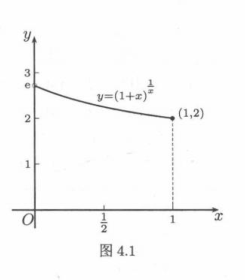
\includegraphics[width=.34\linewidth]{figures/upper/ch04/fig-4-1.png}
\end{center}

对 $x\in(0,1)$，可有 $n\in\NN_+$，使得
\[
  \frac1{n+1}<x\leq\frac1n
\]
成立。实际上将这个不等式改写一下，即是
\[
  n\leq\frac1x<n+1,
\]
可见 $n$ 是由以下公式确定的：
\begin{equation}
  n=\left[\frac1x\right].
  \tag{4.5}
  \label{eq:4.5}
\end{equation}
这时就可以得到估计
\begin{equation}
  \left(1+\frac1{n+1}\right)^n<(1+x)^{1/x}<\left(1+\frac1n\right)^{n+1},
  \tag{4.6}
  \label{eq:4.6}
\end{equation}
其中的 $n$ 由公式 (4.5) 与 $x$ 相联系。若将 $n$ 看成独立的自变量，就有
\[
  \lim_{n\to\infty}\left(1+\frac1{n+1}\right)^n=\ee
  \quad\text{和}\quad
  \lim_{n\to\infty}\left(1+\frac1n\right)^{n+1}=\ee
\]
成立。因此，$\forall\varepsilon>0$，存在 $N$，当 $n>N$ 时，同时成立
\begin{equation}
  \abs{\left(1+\frac1{n+1}\right)^n-\ee}<\varepsilon
  \quad\text{和}\quad
  \abs{\left(1+\frac1n\right)^{n+1}-\ee}<\varepsilon.
  \tag{4.7}
  \label{eq:4.7}
\end{equation}
利用 (4.5)，可见只要有 $0<x<\delta=\frac1{N+1}$，即 $\frac1x>N+1$，就可以使
\[
  n=\left[\frac1x\right]>\frac1x-1>N
\]
成立，从而由 (4.6) 和 (4.7) 得到 $\abs{(1+x)^{1/x}-\ee}<\varepsilon$。这样就证明了
\[
  \lim_{x\to0^+}(1+x)^{1/x}=\ee.
\]
为了讨论 $x\to0^-$，可以取 $z=-x$，则当 $x\to0^-$ 时 $z\to0^+$，因此
\begin{align*}
  \lim_{x\to0^-}(1+x)^{1/x}
  &=\lim_{z\to0^+}(1-z)^{-1/z}
   =\lim_{z\to0^+}\left(\frac1{1-z}\right)^{1/z}\\
  &=\lim_{z\to0^+}\left(1+\frac z{1-z}\right)^{1/z}
   =\lim_{z\to0^+}\left(1+\frac z{1-z}\right)^{\frac{1-z}{z}}
  =\ee.
\end{align*}
合并两个单侧极限就得到所求证的结果。
\end{xproof}

\begin{xremark}
\textbf{注 1}\quad 对 (4.6) 不加分析就直接用夹逼定理是不妥当的。由于该式中间是函数，当然不可能用数列极限的夹逼定理。如果用函数极限的夹逼定理，则 (4.6) 的两侧又是什么样的函数？为什么它们的极限都等于 $\ee$？

实际上该式两侧并非是数列（的通项），而是 $x$ 的函数。它们在每个区间 $[k,k+1)\ (k\in\NN_+)$ 上取常值。若将它们分别记为 $f$ 和 $g$，则先要证明当 $x\to0^+$ 时它们的极限均为 $\ee$，在这以后才可以用函数极限的夹逼定理。读者可以将这个做法与上面从单侧极限的 $\varepsilon$-$\delta$ 定义出发的证明作比较。

\textbf{注 2}\quad 将函数 $(1+x)^{1/x}$ 在 $x=0$ 处补充定义使它连续后，就可以证明延拓后的函数在原点无限次可微。它的 Maclaurin 公式计算见例题 7.2.4。
\end{xremark}

由以上两个重要极限可以导出以下几个基本结果。由于一般教科书中都有它们的证明，这里不再重复。要求读者能记得，会证明：
\begin{enumerate}
  \item $\displaystyle\lim_{x\to0}\frac{\tan x}{x}=1$；
  \item $\displaystyle\lim_{x\to0}\frac{1-\cos x}{x^2}=\frac12$；
  \item $\displaystyle\lim_{x\to0}\frac{\ln(1+x)}x=1$；
  \item $\displaystyle\lim_{x\to0}\frac{a^x-1}{x}=\ln a\quad(a>0)$。
\end{enumerate}

\subsection{例题}

下面的 3 个例题表明，利用复合函数的极限方法，即变量代换法（参见命题 4.1.1），可以扩大以上两个重要极限的适用范围（证明从略）。

\begin{xexample}[4.3.1]
若 $\lim_{t\to t_0}g(t)=0$，且当 $t\ne t_0$ 时 $g(t)\ne0$，则 $\displaystyle\lim_{t\to t_0}\frac{\sin g(t)}{g(t)}=1$。
\end{xexample}

\begin{xexample}[4.3.2]
若 $\lim_{t\to t_0}g(t)=+\infty\ (-\infty)$，则 $\displaystyle\lim_{t\to t_0}\left(1+\frac1{g(t)}\right)^{g(t)}=\ee$。
\end{xexample}

\begin{xexample}[4.3.3]
设 $\lim_{t\to t_0}g(t)=0$，且 $t\ne t_0$ 时 $g(t)\ne0$，则 $\displaystyle\lim_{t\to t_0}\frac{\ln(1+g(t))}{g(t)}=1$。
\end{xexample}

\begin{xexample}[4.3.4]
求 $\displaystyle\lim_{x\to0}(\cos x)^{1/x^2}$。
\end{xexample}
\begin{xsolution}
首先看出这个问题是 $1^\infty$ 型的不定式，因此可以试用上述第一个重要极限。改写原问题如下：
\begin{align*}
  \lim_{x\to0}(\cos x)^{1/x^2}
  &=\lim_{x\to0}\left(1-2\sin^2\frac x2\right)^{1/x^2}\\
  &=\lim_{x\to0}\left(1-2\sin^2\frac x2\right)^{\frac1{-2\sin^2(x/2)}\cdot\frac{-2\sin^2(x/2)}{x^2}}.
\end{align*}
由于
\[
  \lim_{x\to0}\frac{2\sin^2(x/2)}{x^2}
  =\lim_{x\to0}\left(\frac{\sin(x/2)}{x/2}\right)^2\cdot\frac12=\frac12,
\]
因此答案是 $\ee^{-1/2}$。
\end{xsolution}

\begin{xexample}[4.3.5]
求 $\displaystyle\lim_{x\to\infty}\left(\sin\frac1x+\cos\frac1x\right)^x$。
\end{xexample}
\begin{xsolution}
与上一题类似，令
\[
  u_x=\sin\frac1x+\cos\frac1x-1,
\]
则原式可改写为
\[
  \lim_{x\to\infty}(1+u_x)^x
  =\lim_{x\to\infty}\left((1+u_x)^{1/u_x}\right)^{xu_x}.
\]
可见只要计算出
\[
  \lim_{x\to\infty}x\left(\sin\frac1x+\cos\frac1x-1\right)
  =\lim_{x\to\infty}\left(\frac{\sin(1/x)}{1/x}-\frac{2\sin^2(1/(2x))}{(1/(2x))\cdot2}\right)=1,
\]
即知原问题的答案为 $\ee$。
\end{xsolution}

\begin{xremark}
以上两个例题的求解在写法上可以利用 $u^v=\ee^{v\ln u}$ 和例题 4.3.3 改写如下（只写出后一例题）：
\begin{align*}
  \lim_{x\to\infty}x\ln\left(\sin\frac1x+\cos\frac1x\right)
  &=\lim_{x\to\infty}x\ln\left[1+\left(\sin\frac1x+\cos\frac1x-1\right)\right]\\
  &=\lim_{x\to\infty}x\left(\sin\frac1x+\cos\frac1x-1\right),
\end{align*}
以下同上。又如果一开始作代换 $y=1/x$，则在书写上更方便一些。
\end{xremark}

\subsection{练习题}

\begin{xexercise}[1]
计算下列极限：
  \begin{enumerate}
    \item $\displaystyle\lim_{x\to+\infty}\left(\frac2\pi\arctan x\right)^x$；
    \item $\displaystyle\lim_{x\to\pi/2}(\sin x)^{\tan x}$；
    \item $\displaystyle\lim_{x\to\infty}\left(\frac{x^2-1}{x^2+1}\right)^{x^2}$；
    \item $\displaystyle\lim_{x\to\pi/2^-}(\cos x)^{\frac\pi2-x}$；
    \item $\displaystyle\lim_{x\to0}\frac{\sin2x-2\sin x}{x^3}$；
    \item $\displaystyle\lim_{x\to1}(1-x)\tan\left(\frac\pi2x\right)$。
  \end{enumerate}
\end{xexercise}
\begin{xsolution}
由
\[
  \frac{\tan x}{x}=\frac{\sin x}{x}\cdot\frac1{\cos x}
\]
及 $\sin x/x\to1$、$\cos x\to1$，得
$\lim_{x\to0}\tan x/x=1$。

\begin{enumerate}[label=(\arabic*)]
  \item 利用 $\arctan x=\pi/2-\arctan(1/x)$，令
  $u=(2/\pi)\arctan(1/x)\sim2/(\pi x)$。则
  \[
    x\ln\left(\frac2\pi\arctan x\right)
    =x\ln(1-u)\to-\frac2\pi,
  \]
  故极限为 $\ee^{-2/\pi}$。

  \item 令 $h=x-\pi/2$。则
  $\sin x=\cos h=1-\frac12h^2+\littleo(h^2)$，且
  $\tan x=-\cot h\sim-1/h$。所以
  \[
    \tan x\,\ln(\sin x)
    \sim\left(-\frac1h\right)\left(-\frac12h^2\right)\to0,
  \]
  原极限为 1。

  \item
  \[
    x^2\ln\frac{x^2-1}{x^2+1}
    =x^2\ln\left(1-\frac2{x^2+1}\right)\to-2,
  \]
  故极限为 $\ee^{-2}$。

  \item 令 $h=\pi/2-x\to0^+$，则 $\cos x=\sin h$，故
  \[
    \ln\bigl((\cos x)^{\pi/2-x}\bigr)=h\ln(\sin h)
    =h\ln h+h\ln\frac{\sin h}{h}\to0.
  \]
  因而极限为 1。

  \item
  \[
    \frac{\sin2x-2\sin x}{x^3}
    =2\frac{\sin x}{x}\frac{\cos x-1}{x^2}\to2\cdot1\cdot\left(-\frac12\right)=-1.
  \]

  \item 令 $h=1-x\to0$，则
  \[
    (1-x)\tan\frac{\pi x}{2}
    =h\cot\frac{\pi h}{2}
    =\frac2\pi\frac{(\pi h/2)}{\tan(\pi h/2)}\to\frac2\pi.
  \]
\end{enumerate}
\end{xsolution}


\begin{xexercise}[2]
注意下列两个“不等式”并求出正确值：
  \begin{enumerate}
    \item $\displaystyle\lim_{x\to+\infty}\frac{\sin x}{x}\ne1$；
    \item $\displaystyle\lim_{x\to+\infty}(1+x)^{1/x}\ne\ee$。
  \end{enumerate}
\end{xexercise}
\begin{xsolution}
利用 $1-\cos x=2\sin^2(x/2)$，
\[
  \frac{1-\cos x}{x^2}
  =\frac12\left(\frac{\sin(x/2)}{x/2}\right)^2\to\frac12.
\]

(1) 由于 $\abs{\sin x}\leq1$，
\[
  \abs{\frac{\sin x}{x}}\leq\frac1x\to0,
\]
故正确值是 0。

(2) 取对数：
\[
  \ln\bigl((1+x)^{1/x}\bigr)=\frac{\ln(1+x)}x\to0
  \qquad(x\to+\infty),
\]
因为 $\ln(1+x)=\littleo(x)$。故正确值是 1。
\end{xsolution}


\begin{xexercise}[3]
设 $a>0,b>0$，求极限
  \[
    \lim_{n\to\infty}\left(\frac{\sqrt[n]{a}+\sqrt[n]{b}}2\right)^n.
  \]
  （本题是数列极限问题，但现在可以用函数极限知识来解决。）
\end{xexercise}
\begin{xsolution}
由第二个重要极限
$(1+x)^{1/x}\to\ee$，并利用 $\ln$ 的连续性，
\[
  \frac{\ln(1+x)}x
  =\ln\bigl((1+x)^{1/x}\bigr)\to\ln\ee=1.
\]

由
\[
  a^{1/n}=1+\frac{\ln a}{n}+\littleo\left(\frac1n\right),\qquad
  b^{1/n}=1+\frac{\ln b}{n}+\littleo\left(\frac1n\right),
\]
可得
\[
  \frac{a^{1/n}+b^{1/n}}2
  =1+\frac{\ln a+\ln b}{2n}+\littleo\left(\frac1n\right).
\]
于是
\[
  \left(\frac{a^{1/n}+b^{1/n}}2\right)^n
  \to\exp\left(\frac{\ln a+\ln b}{2}\right)=\sqrt{ab}.
\]
\end{xsolution}


\begin{xexercise}[4]
设 $a_1,\ldots,a_n$ 为正数，$n\geq2$，
  \[
    f(x)=\left(\frac{a_1^x+a_2^x+\cdots+a_n^x}{n}\right)^{1/x},
  \]
  求 $\displaystyle\lim_{x\to0}f(x)$。
\end{xexercise}
\begin{xsolution}
若 $a=1$，结论显然为 0。设 $a>0,a\ne1$，令 $y=a^x-1$，则 $y\to0$，且
$\ln(1+y)=x\ln a$。于是
\[
  \frac{a^x-1}{x}
  =\ln a\,\frac{y}{\ln(1+y)}\to\ln a.
\]

对每个 $i$，
\[
  a_i^x=\ee^{x\ln a_i}=1+x\ln a_i+\littleo(x).
\]
因此
\[
  \frac1n\sum_{i=1}^n a_i^x
  =1+x\left(\frac1n\sum_{i=1}^n\ln a_i\right)+\littleo(x).
\]
记 $c=\frac1n\sum\ln a_i$，则
\[
  \ln f(x)=\frac1x\ln(1+cx+\littleo(x))\to c.
\]
故
\[
  \lim_{x\to0}f(x)=\ee^c=(a_1a_2\cdots a_n)^{1/n}.
\]
\end{xsolution}


\begin{xexercise}[5]
计算极限 $\displaystyle\lim_{n\to\infty}\prod_{k=1}^n\cos\frac{x}{2^k}$，并证明 Viète（韦达）公式
  \[
    \frac\pi2=
    \frac{1}{
      \sqrt{\frac12}\cdot
      \sqrt{\frac12+\frac12\sqrt{\frac12}}\cdot
      \sqrt{\frac12+\frac12\sqrt{\frac12+\frac12\sqrt{\frac12+\cdots}}}}
    .
  \]

  （这是数学家 Viète 在 1593 年发表的。它是数学史上第一次用无穷乘积来表示一个数，同时也是对于圆周率 $\pi$ 的认识上的重大突破。）
\end{xexercise}
\begin{xsolution}
反复使用 $\sin u=2\sin(u/2)\cos(u/2)$，得到
\[
  \sin x=2^n\sin\frac{x}{2^n}\prod_{k=1}^n\cos\frac{x}{2^k}.
\]
因此对固定 $x$，
\[
  \prod_{k=1}^n\cos\frac{x}{2^k}
  =\frac{\sin x}{2^n\sin(x/2^n)}
  =\frac{\sin x}{x}\cdot\frac{x/2^n}{\sin(x/2^n)}
  \to\frac{\sin x}{x},
\]
在 $x=0$ 时按连续延拓理解为 1。

取 $x=\pi/2$，得
\[
  \prod_{k=1}^{\infty}\cos\frac{\pi}{2^{k+1}}=\frac2\pi.
\]
而半角公式依次给出
\[
  \cos\frac\pi4=\sqrt{\frac12},
  \quad
  \cos\frac\pi8=\sqrt{\frac12+\frac12\sqrt{\frac12}},
\]
并继续产生题中嵌套根式。取上式倒数即得 Viète 公式。
\end{xsolution}


\section{无穷小量、有界量、无穷大量和阶的比较}

从数列开始，就已接触到无穷小量、有界量和无穷大量的概念。在本节将介绍如何将它们用于函数极限计算，其中特别是等价量代换法将成为计算函数极限的基本方法之一。

\subsection{\texorpdfstring{记号 $\littleo,\bigO$ 与 $\sim$}{记号 o、O 与渐近等价}}

设 $f(x)$ 和 $g(x)$ 在点 $a$ 的某个去心邻域 $O(a)-\{a\}$ 上定义，并且 $g(x)\ne0$。（对于 $a$ 为无穷大量的情况和单侧极限等情况可类推。）

\begin{enumerate}
  \item $f(x)=\littleo(g(x))\ (x\to a)$ 的定义是：$\displaystyle\lim_{x\to a}\frac{f(x)}{g(x)}=0$，如果当 $x\to a$ 时 $f(x)$ 和 $g(x)$ 都是无穷小量，则称当 $x\to a$ 时 $f(x)$ 是比 $g(x)$ 更高阶的无穷小量。
  \item $f(x)=\littleo(1)\ (x\to a)$ 的定义是：$\displaystyle\lim_{x\to a}f(x)=0$。因此与数列情况一样，记号 $\littleo(1)$ 用于表示关于某个极限过程的无穷小量。
  \item $f(x)=\bigO(g(x))\ (x\to a)$ 的定义是：存在常数 $M>0$，使得 $\displaystyle\abs{\frac{f(x)}{g(x)}}\leq M$ 在 $a$ 的某个去心邻域上成立，因此成立不等式 $\abs{f(x)}\leq M\abs{g(x)}$。
  \item $f(x)=\bigO(1)\ (x\to a)$ 的定义是：存在 $a$ 的某个去心邻域，使 $f$ 在其上有界。这与数列情况不太一样，在那里 $\bigO(1)$ 就是有界量，而在这里记号 $\bigO(1)\ (x\to a)$ 用于表示在点 $a$ 的某个去心邻域上的一个有界量，因此也称为局部有界量。
  \item 如果有 $\displaystyle\lim_{x\to a}\frac{f(x)}{g(x)}=A\ne0$，而且当 $x\to a$ 时 $f$ 和 $g$ 都是无穷小量（无穷大量），则称 $f$ 和 $g$ 是同阶无穷小量（无穷大量）。
  \item $f(x)\sim g(x)\ (x\to a)$ 的定义是：$\displaystyle\lim_{x\to a}\frac{f(x)}{g(x)}=1$，如果当 $x\to a$ 时 $f$ 和 $g$ 是无穷小量（无穷大量），则称 $f$ 和 $g$ 是等价无穷小量（无穷大量）。
\end{enumerate}

今后我们还将含有 $\littleo,\bigO$ 和 $\sim$ 的等式称为渐近等式，并将 $f(x)\sim g(x)\ (x\to a)$ 说成是函数 $f(x)$ 和 $g(x)$ 当 $x\to a$ 时具有相同的渐近性态。特别是当 $x\to\infty$（包括数列极限中的 $n\to\infty$）时这种表述在数学中用得很广泛。

\begin{enumerate}[start=7]
  \item 以上所说有关阶的概念还可以量化，其方法是对有关的极限过程取一类简单的无穷小量（或无穷大量）作为标准。下面只举出常用的情况。设已知 $f(x)=\littleo(1)\ (x\to a)$。若有常数 $\alpha>0$，使得
  \[
    \lim_{x\to a}\abs{\frac{f(x)}{(x-a)^\alpha}}=l>0,
  \]
  则称 $f(x)$ 在 $x\to a$ 时是 $\alpha$ 阶的无穷小量。
  \item 在使用这些记号时，必需写出有关的极限过程。除了对数列可以不写出 $(n\to\infty)$ 外，其他极限过程均不可省略（除非另加说明）。例如以下关于对数函数的三个最基本的渐近性质当然是与相应的极限过程不可分开的：
  \[
    \ln x=\littleo(1)\ (x\to1),\qquad
    \ln x=\littleo(x)\ (x\to+\infty),\qquad
    \ln x=\littleo\left(\frac1x\right)\ (x\to0^+).
  \]
  \item 下面是几个重要的极限关系（其中题 (7) 见下面的例题 4.4.4）：
  \begin{enumerate}
    \item $\ee^x-1\sim x\ (x\to0)$；
    \item $\sin x\sim x\ (x\to0)$；
    \item $\ln(1+x)\sim x\ (x\to0)$；
    \item $1-\cos x\sim\frac12x^2\ (x\to0)$；
    \item $\ln x=\littleo(x^{-\alpha})\ (x\to0^+)\ (\alpha>0)$；
    \item $x^k=\littleo(a^x)\ (x\to+\infty)\ (a>1)$；
    \item $(1+x)^\alpha-1\sim\alpha x\ (x\to0)$；
    \item $\arctan x\sim x\ (x\to0)$。
  \end{enumerate}
\end{enumerate}

上面引进的一些记号，即 $\littleo,\bigO,\sim$ 和关于阶与等价的概念在处理函数极限时是很有用的工具，但这里对初学者来说同时也有许多陷阱，很容易出错。

在使用 $\littleo,\bigO,\sim$ 时，除了必须写明极限过程之外，还要知道以下两点：

首先，含有 $\littleo,\bigO$ 的等式，即渐近等式，与普通的等式大不一样。它们并不是量的相等，而是代表在极限过程中的关系。

其次，它们一般只能从左往右读，而不能从右往左读。例如 $\littleo(1)=\bigO(1)\ (x\to a)$ 的含义是：无穷小量必是局部有界量。而 $\bigO(1)=\littleo(1)\ (x\to a)$ 是错的，因为局部有界量当然未必是无穷小量。

\begin{xremark}
含有 $\littleo,\bigO$ 的等式，是大部分学生理解的难点。从数学中，我们发现从集合论的角度，可以向学生说清楚这种等式的真正含义。例如，在 $x\to0$ 时，将 $\littleo(x)$ 理解为比 $x$ 高阶的无穷小量组成的集合，于是等式 $f(x)=\littleo(x)$ 中等号 = 所实际表达的意思是 $\in$。凡是只有右边含有 $\littleo,\bigO$ 的等式都可以这样理解。而两边都含有 $\littleo,\bigO$ 的等式中的等号 = 实际表达的意思是 $\subset$。因此，它们只能从左往右读。
\end{xremark}

\begin{xexample}[4.4.1]
证明 $\bigO(x^2)=\littleo(x)\ (x\to0)$。
\end{xexample}
\begin{xproof}
根据题意，设 $\dfrac{f(x)}{x^2}$ 在某个 $O(0)-\{0\}$ 上有界，即存在 $M>0$ 和 $\delta>0$，当 $0<\abs{x}<\delta$ 时，成立 $\abs{f(x)}\leq Mx^2$。于是，当 $0<\abs{x}<\delta$ 时，有
\[
  \abs{\frac{f(x)}x}\leq\abs{\frac{Mx^2}x}=\abs{Mx},
\]
因此，令 $x\to0$ 时，上式的极限为 0。这就是 $f(x)=\littleo(x)\ (x\to0)$。这样我们就证明了当 $f(x)=\bigO(x^2)\ (x\to0)$ 时，一定就有 $f(x)=\littleo(x)\ (x\to0)$。
\end{xproof}

\begin{xexample}[4.4.2]
证明 $\cos x=1+\bigO(x^2)\ (x\to0)$ 成立。
\end{xexample}
\begin{xproof}
已知有 $\displaystyle\lim_{x\to0}\frac{1-\cos x}{x^2}=\frac12$，因此存在 $\delta>0$，使得当 $0<\abs{x}<\delta$ 时，$\dfrac{\cos x-1}{x^2}$ 有界。这就是说 $\cos x-1=\bigO(x^2)\ (x\to0)$。再移项即得。
\end{xproof}

关于无穷小量的阶可以从前面的许多例子得到理解。例如，当 $x\to0$ 时，$\sin x$ 是一阶无穷小量，$1-\cos x$ 是二阶无穷小量，$\sin x-\tan x$ 是三阶无穷小量等（后者见例题 4.4.5）。又由此可见 $\sin x=\bigO(x)$，$1-\cos x=\bigO(x^2)$，$\sin x-\tan x=\bigO(x^3)\ (x\to0)$，但并不能从这三个公式推出关于阶的结论。

应当指出，无穷小量（以及无穷大量）不一定有阶。

\begin{xexample}[4.4.3]
证明：当 $x\to0$ 时无穷小量 $x\sin\frac1x$ 没有阶。
\end{xexample}
\begin{xproof}
这只要观察
\[
  \lim_{x\to0}\frac{x\sin\frac1x}{x^\alpha}
\]
即可。如取 $\alpha\geq1$，则上述极限不存在，但若取 $\alpha<1$，则上述极限为 0，因此没有阶。但是也可以说它的阶比任何 $\alpha<1$ 高。
\end{xproof}

当然有 $x\sin\frac1x=\bigO(x)$，$x\sin\frac1x=\littleo(x^\alpha),\forall\alpha<1\ (x\to0)$。

最后再举出两个用等价记号 $\sim$ 刻画的重要渐近公式。

\begin{enumerate}
  \item 关于阶乘的 Stirling 公式：
  \[
    n!\sim\left(\frac n\ee\right)^n\sqrt{2\pi n}.
  \]
  它的证明将在积分学中给出（命题 11.4.2）。
  \item 如果将不超过 $x$ 的素数个数记为 $\pi(x)$，则有素数定理：
  \[
    \pi(x)\sim\frac{x}{\ln x}\quad(x\to+\infty).
  \]
  素数定理是数论中的重要定理。Legendre（勒让德）和 Gauss 通过实验提出了猜测。Hadamard（阿达马）和 de la Vallée-Poussin（德拉瓦莱普森）于 1896 年分别独立地给出了素数定理的第一个证明。1949 年，Selberg（塞尔伯格）和 Erdös（爱尔迪希）又给出了它的初等证明。（例如可参考华罗庚的《数论导引》。）
\end{enumerate}

\subsection{思考题}

\begin{xthought}[1]
$10^{-10,000},\ee^{-10^{10}},x,\sin x$ 是否是无穷小量？$10^{10,000},\ee^{10^{10}},x^n,a^x\ (a>1)$ 是否是无穷大量？
\end{xthought}
\begin{xsolution}
“无穷小量”“无穷大量”都必须依附于一个极限过程，不能只看数值的绝对大小。因此固定常数
$10^{-10000}$、$\ee^{-10^{10}}$ 虽然很小，仍只是非零常数，不是无穷小量；固定常数
$10^{10000}$、$\ee^{10^{10}}$ 虽然很大，仍是有限数，不是无穷大量。

$x$、$\sin x$ 是否为无穷小量要看极限过程。例如 $x\to0$ 时两者都是无穷小量，而 $x\to+\infty$ 时 $x$ 不是无穷小量，$\sin x$ 也不趋于 0。类似地，$x^n$、$a^x$（$a>1$）在 $x\to+\infty$ 时是无穷大量，但在别的极限过程中未必如此。
\end{xsolution}


\begin{xthought}[2]
确定下列极限是否存在，若存在，等于什么？（观察图 4.2 中的图像。）
  \begin{enumerate}
    \item $\displaystyle\lim_{x\to0}\frac{\sin x}{x}$；
    \item $\displaystyle\lim_{x\to+\infty}\frac{\sin x}{x}$；
    \item $\displaystyle\lim_{x\to0}x\sin\frac1x$；
    \item $\displaystyle\lim_{x\to\infty}x\sin\frac1x$；
    \item $\displaystyle\lim_{x\to0}x\sin x$；
    \item $\displaystyle\lim_{x\to\infty}x\sin x$；
    \item $\displaystyle\lim_{x\to0}\frac1x\sin\frac1x$；
    \item $\displaystyle\lim_{x\to\infty}\frac1x\sin\frac1x$。
  \end{enumerate}

  \begin{center}
    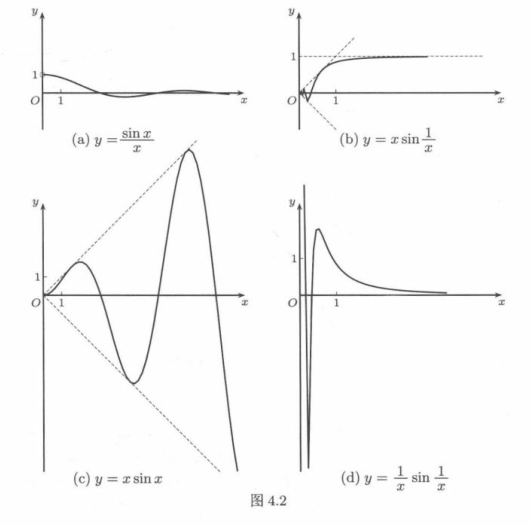
\includegraphics[width=.70\linewidth]{figures/upper/ch04/fig-4-2.png}
  \end{center}
\end{xthought}
\begin{xsolution}
\begin{enumerate}[label=(\arabic*)]
  \item $\displaystyle\lim_{x\to0}\frac{\sin x}{x}=1$。
  \item $\displaystyle\lim_{x\to+\infty}\frac{\sin x}{x}=0$，因为绝对值不超过 $1/x$。
  \item $\displaystyle\lim_{x\to0}x\sin\frac1x=0$，因为绝对值不超过 $\abs x$。
  \item $\displaystyle\lim_{x\to\infty}x\sin\frac1x=1$，因为令 $t=1/x\to0$ 后
  $x\sin(1/x)=\sin t/t\to1$。
  \item $\displaystyle\lim_{x\to0}x\sin x=0$，例如 $\abs{x\sin x}\leq\abs x$。
  \item $\displaystyle\lim_{x\to\infty}x\sin x$ 不存在。沿 $x_n=n\pi$ 值恒为 0；沿
  $y_n=2n\pi+\pi/2$，值 $y_n\to+\infty$。
  \item $\displaystyle\lim_{x\to0}\frac1x\sin\frac1x$ 不存在。沿 $x_n=1/(n\pi)$ 值为 0；沿
  $y_n=1/(2n\pi+\pi/2)$，值为 $2n\pi+\pi/2\to+\infty$。
  \item $\displaystyle\lim_{x\to\infty}\frac1x\sin\frac1x=0$。令 $t=1/x$，则
  $t\sin t\to0$。
\end{enumerate}
\end{xsolution}


\begin{xthought}[3]
当 $x\to0$ 时，下列等式中哪些可以成立：
  \begin{enumerate}
    \item $\littleo(1)=\bigO(1)$；
    \item $\bigO(1)=\littleo(1)$；
    \item $\littleo(x^2)=\littleo(x)$；
    \item $\bigO(x^2)=\littleo(x)$；
    \item $x\cdot\littleo(x^2)=\littleo(x^3)$；
    \item $\dfrac{\bigO(x^2)}x=\littleo(x)$。
  \end{enumerate}
\end{xthought}
\begin{xsolution}
这些式子中的等号按本章约定表示相应函数类的包含关系。
\begin{enumerate}[label=(\arabic*)]
  \item 可以。$\littleo(1)\subset\bigO(1)$，因为无穷小量必局部有界。
  \item 不可以。例如常函数 1 属于 $\bigO(1)$，但不属于 $\littleo(1)$。
  \item 可以。若 $f=\littleo(x^2)$，则
  \[
    \frac{f(x)}x=\frac{f(x)}{x^2}x\to0,
  \]
  故 $f=\littleo(x)$。
  \item 可以。若 $f=\bigO(x^2)$，则 $\abs{f(x)}\leq Cx^2$，从而
  $\abs{f(x)/x}\leq C\abs x\to0$，故 $f=\littleo(x)$。
  \item 可以。若 $r(x)=\littleo(x^2)$，则
  \[
    \frac{x r(x)}{x^3}=\frac{r(x)}{x^2}\to0,
  \]
  故 $x\littleo(x^2)=\littleo(x^3)$。
  \item 不可以。由 $f=\bigO(x^2)$ 只能推出 $f/x=\bigO(x)$。取 $f(x)=x^2$，则
  $f(x)/x=x$，而 $x$ 不是 $\littleo(x)$。
\end{enumerate}
\end{xsolution}


\begin{xthought}[4]
作出 $y=\ee^{1/x}$ 的图形，观察：$\ee^{1/x}\to+\infty\ (x\to0^+)$ 和 $\ee^{1/x}=\littleo(1)\ (x\to0^-)$。
\end{xthought}
\begin{xsolution}
函数 $y=\ee^{1/x}$ 在 $x=0$ 两侧分别形成两支。对 $x>0$，当 $x\to0^+$ 时 $1/x\to+\infty$，故
\[
  \ee^{1/x}\to+\infty.
\]
对 $x<0$，当 $x\to0^-$ 时 $1/x\to-\infty$，故
\[
  \ee^{1/x}\to0,
\]
也就是 $\ee^{1/x}=\littleo(1)$（$x\to0^-$）。此外 $x\to\pm\infty$ 时 $\ee^{1/x}\to1$，所以图像在两端都以 $y=1$ 为水平渐近线。
\end{xsolution}


\subsection{等价量代换法}

在求极限的计算中，等价量代换法是基本方法之一。

\begin{xexample}[4.4.4]
设 $\alpha\ne0$。求 $\displaystyle\lim_{x\to0}\frac{(1+x)^\alpha-1}{x}$。
\end{xexample}
\begin{xsolution}
令 $y=(1+x)^\alpha-1$，则当 $x\to0$ 时 $y\to0$。利用 $1+y=(1+x)^\alpha$，有 $\ln(1+y)=\alpha\ln(1+x)$。计算如下：
\[
  \lim_{x\to0}\frac{(1+x)^\alpha-1}{x}
  =\lim_{x\to0}\frac{(1+x)^\alpha-1}{\ln(1+x)}
  =\lim_{y\to0}\frac{\alpha y}{\ln(1+y)}
  =\lim_{y\to0}\frac{\alpha y}{y}=\alpha.
\]
\end{xsolution}

\begin{xremark}
\textbf{注 1}\quad 本例是变量代换和等价量代换两个方法结合的典型例子。在以上计算中先利用 $\ln(1+x)\sim x\ (x\to0)$，将分母的 $x$ 换为 $\ln(1+x)$（将简单换成复杂），后来又利用 $\ln(1+y)\sim y\ (y\to0)$，将 $\ln(1+y)$ 换为 $y$。

\textbf{注 2}\quad 在本例中的指数 $\alpha$ 可以是不为 0 的任何实数。而在过去我们只能用二项式展开的方法处理 $\alpha$ 为有理数的情况。今后可以直接应用本题的一般结论。
\end{xremark}

\begin{xexample}[4.4.5]
求极限 $\displaystyle\lim_{x\to0}\frac{\sin x-\tan x}{x^3}$。
\end{xexample}
\begin{xsolution}
\textbf{解 1}\quad 将表达式进行分解，利用已知极限即可如下计算：
\[
  \lim_{x\to0}\frac{\sin x-\tan x}{x^3}
  =\lim_{x\to0}\left(\frac{\sin x}{x}\cdot\frac1{\cos x}\cdot\frac{\cos x-1}{x^2}\right)
  =-\frac12.
\]

\textbf{解 2}\quad 若用等价量代换法，则可写出
\[
  \frac{\sin x-\tan x}{x^3}=\frac{\sin x(\cos x-1)}{x^3\cos x},
\]
然后利用当 $x\to0$ 时的等价关系 $\sin x\sim x$，$1-\cos x\sim\frac12x^2$ 和 $\cos x\sim1$，将上面的表达式中的 $\sin x$ 换为 $x$，$\cos x$ 换为 1，$\cos x-1$ 换为 $-\frac12x^2$，就有
\[
  \lim_{x\to0}\frac{\sin x-\tan x}{x^3}
  =\lim_{x\to0}\frac{\sin x(\cos x-1)}{x^3\cos x}
  =\lim_{x\to0}\frac{x(-\frac12x^2)}{x^3}=-\frac12.
\]
\end{xsolution}

\paragraph{小结}
一般的等价量代换法可以叙述如下：

设要求极限 $\lim_{x\to a}uv$，其中 $u,v$ 是 $x$ 的函数。如已知 $u\sim u_1\ (x\to a)$，则可以将上式中的因子 $u$ 用 $u_1$ 代替，写成公式就是
\begin{equation}
  \lim_{x\to a}uv
  =\lim_{x\to a}\left(\frac u{u_1}\right)u_1v
  =\lim_{x\to a}u_1v,
  \tag{4.8}
  \label{eq:4.8}
\end{equation}
这就是说可以将 $u$ 换成 $u_1$（其中假定在 $a$ 邻近 $u_1\ne0$）。当然这个做法可以反复使用，例如在例题 4.4.5 的解 2 中就代换了三个因子，使函数的表达式大大简化。

在这里要强调指出：在对于形式为 $u+v$ 或 $(u+v)w$ 的函数求极限时，即使有 $u\sim u_1$ 也不能将 $u$ 随便换成 $u_1$。例如在例题 4.4.5 中，以下做法都是错误的：
\begin{enumerate}
  \item 利用 $\sin x\sim\tan x\ (x\to0)$ 得到 $\displaystyle\lim_{x\to0}\frac{\sin x-\tan x}{x^3}=\lim_{x\to0}\frac{\sin x-\sin x}{x^3}=0$。
  \item 利用 $\sin x\sim x\ (x\to0)$ 得到 $\displaystyle\lim_{x\to0}\frac{\sin x-\tan x}{x^3}=\lim_{x\to0}\frac{x-\tan x}{x^3}=-\frac13$。
  \item 利用 $\tan x\sim x\ (x\to0)$ 得到 $\displaystyle\lim_{x\to0}\frac{\sin x-\tan x}{x^3}=\lim_{x\to0}\frac{\sin x-x}{x^3}=-\frac16$。
\end{enumerate}
这三个例子中的最后一步都没有错（其中后两个数值 $-\frac13$ 和 $-\frac16$ 的计算在学了微分学后就可以得到），但答案都是错的。其原因是第一步的代换没有根据。

什么条件下才可以在和式中用等价量代换？

假定考虑的极限过程为 $x\to a$，则一个容易证明的充分条件就是
\begin{equation}
  u\sim u_1,\ v\sim v_1,\ \lim_{x\to a}u+v\ne0
  \quad\Longrightarrow\quad u+v\sim u_1+v_1.
  \tag{4.9}
  \label{eq:4.9}
\end{equation}
它清楚地表明，在和式中用等价量代换出错的根源就在于当时起作用的是更高阶的无穷小量。关于 (4.9) 的证明从略。这方面有许多研究，感兴趣的读者可以参考 [57] 以及其中所引的文献。

实际上等价量代换（在无穷小量的情况）的本质就是用较为简单的无穷小量代替比较复杂的无穷小量，而将两个无穷小量之间的差略去不计。当然，这时它们的差必须是更高阶的无穷小量。一种安全的做法就是保留高阶无穷小量，而不是简单的代换。从下一个例题中可以看到这是如何进行的。

\begin{xexample}[4.4.6]
设 $f(x)=\dfrac{m}{1-x^m}-\dfrac{n}{1-x^n}$，$m,n\in\NN_+$，求极限 $\displaystyle\lim_{x\to1}f(x)$。
\end{xexample}
\begin{xsolution}
令 $y=x-1$，则 $x\to1\Longleftrightarrow y\to0$。计算如下：
\begin{align*}
  f(x)=f(1+y)
  &=\frac{m}{1-(1+y)^m}-\frac{n}{1-(1+y)^n}\\
  &=\frac{m[1-(1+y)^n]-n[1-(1+y)^m]}
          {[(1+y)^m-1]\cdot[(1+y)^n-1]}\\
  &=\frac{n\left[my+\frac{m(m-1)}2y^2+\littleo(y^2)\right]
          -m\left[ny+\frac{n(n-1)}2y^2+\littleo(y^2)\right]}
          {mn(y+\littleo(y))\cdot(y+\littleo(y))}\\
  &=\frac{\frac{mn}2(m-n)y^2+\littleo(y^2)}{mn(y^2+\littleo(y^2))}
   =\frac12(m-n)+\littleo(1)\quad(y\to0),
\end{align*}
其中的 $\littleo(y^2),\littleo(y),\littleo(1)$ 均是对 $y\to0$ 而言的，可见极限为 $\frac12(m-n)$。
\end{xsolution}

\begin{xremark}
以上所用的方法已经超出了等价量代换法的思想。一般称
\[
  (1+y)^n=1+ny+\littleo(y)\quad(y\to0)
\]
或
\[
% SOURCE-ERR: 原书此式在 n(n-1)/2 后漏印 y^2；由二项展开及上文计算可确定应补入。
  (1+y)^n=1+ny+\frac{n(n-1)}2y^2+\littleo(y^2)\quad(y\to0)
\]
中的 $\littleo(y)$ 或 $\littleo(y^2)$ 为余项。在上一个例题中出现的各个余项是根据需要而分别选取的。在今后学习微分学中带 Peano（佩亚诺）余项的 Taylor 公式后（见命题 7.2.2），可以将这个例题中的方法发展成更一般的方法（见 §8.1 “函数极限的计算”）。
\end{xremark}

\subsection{练习题}

\begin{xexercise}[1]
确定下列无穷小量的阶：
  \begin{enumerate}
    \item $\sqrt{1+\tan x}-\sqrt{1-\tan x}\ (x\to0)$；
    \item $\ln x-\ln a\ (x\to a),a>0$；
    \item $a^{x^2}-1\ (x\to0)$，其中 $a>0$；
    \item $a^{x^2}-b^{x^2}\ (x\to0)$，其中 $a,b>0$；
    \item $\ln\left(x+\cos\frac\pi2x\right)\ (x\to1)$；
    \item $\ln x\ln(x-1)\ (x\to1^+)$。
  \end{enumerate}
\end{xexercise}
\begin{xsolution}
\begin{enumerate}[label=(\arabic*)]
  \item
  \[
    \sqrt{1+\tan x}-\sqrt{1-\tan x}
    =\frac{2\tan x}{\sqrt{1+\tan x}+\sqrt{1-\tan x}}
    \sim x.
  \]
  因而是一阶无穷小量。

  \item
  \[
    \ln x-\ln a=\ln\left(1+\frac{x-a}{a}\right)
    \sim\frac{x-a}{a},
  \]
  因而是一阶无穷小量。

  \item
  \[
    a^{x^2}-1=(\ln a)x^2+\littleo(x^2).
  \]
  若 $a\ne1$，则 $\ln a\ne0$，所以它是二阶无穷小量；若 $a=1$，函数恒为 0，不具有题目定义下的有限正阶，可视为高于任意有限阶。

  \item
  \[
    a^{x^2}-b^{x^2}
    =(\ln a-\ln b)x^2+\littleo(x^2).
  \]
  若 $a\ne b$，是二阶无穷小量；若 $a=b$，恒为 0，不具有有限正阶。

  \item 令 $h=x-1$。有
  \[
    x+\cos\frac{\pi x}{2}
    =1+h-\sin\frac{\pi h}{2}
    =1+\left(1-\frac\pi2\right)h+\littleo(h).
  \]
  因此
  \[
    \ln\left(x+\cos\frac{\pi x}{2}\right)
    \sim\left(1-\frac\pi2\right)(x-1),
  \]
  是一阶无穷小量。

  \item 令 $h=x-1\to0^+$。则
  \[
    \ln x\ln(x-1)=\ln(1+h)\ln h\sim h\ln h\to0.
  \]
  对任意 $\alpha<1$，$h^{1-\alpha}\ln h\to0$；对 $\alpha=1$，商为 $\ln h\to-\infty$；对 $\alpha>1$，商的绝对值也趋于无穷。因此不存在 $\alpha>0$ 使与 $h^\alpha$ 的商趋于非零有限数，即该无穷小量没有阶；但它比任意 $\alpha<1$ 阶无穷小量更高阶。
\end{enumerate}
\end{xsolution}


\begin{xexercise}[2]
设存在极限 $\displaystyle\lim_{x\to0}\frac{f(x)}x$，又有 $f(x)-f\left(\frac x2\right)=\littleo(x)\ (x\to0)$，证明：$f(x)=\littleo(x)\ (x\to0)$。
\end{xexercise}
\begin{xsolution}
设
\[
  L=\lim_{x\to0}\frac{f(x)}x.
\]
则
\[
  f(x)=Lx+\littleo(x),
  \qquad
  f\left(\frac x2\right)=\frac L2x+\littleo(x).
\]
相减得
\[
  f(x)-f\left(\frac x2\right)=\frac L2x+\littleo(x).
\]
题设左端为 $\littleo(x)$，两边除以 $x$ 后令 $x\to0$，得到 $L/2=0$，故 $L=0$。于是
$f(x)/x\to0$，即 $f(x)=\littleo(x)$。
\end{xsolution}


\begin{xexercise}[3]
与数列中的几个常见的无穷大量之间的关系 $\ln n\ll n^\varepsilon\ll a^n\ll n!\ll n^n\ (a>1,\varepsilon>0)$ 相类似，证明当 $x\to+\infty$ 时，有
  \[
    \ln x\ll x^\varepsilon\ll a^x\ll x^x\quad(a>1,\varepsilon>0),
  \]
  其中 $u\ll v$ 的定义是 $\displaystyle\lim\frac uv=0$。
\end{xexercise}
\begin{xsolution}
第一层关系由 4.2.5 题 1(2) 直接得到：
\[
  \frac{\ln x}{x^\varepsilon}\to0.
\]
第二层由 4.2.5 题 1(1) 得到：
\[
  \frac{x^\varepsilon}{a^x}\to0\qquad(a>1).
\]
最后
\[
  \frac{a^x}{x^x}
  =\exp\bigl(x\ln a-x\ln x\bigr)
  =\exp\bigl(-x(\ln x-\ln a)\bigr)\to0,
\]
因为 $\ln x-\ln a\to+\infty$。故
\[
  \ln x\ll x^\varepsilon\ll a^x\ll x^x.
\]
\end{xsolution}


\begin{xexercise}[4]
用等价量代换方法计算下列极限：
  \begin{enumerate}
    \item $\displaystyle\lim_{x\to0}\frac{\ln(\sin^2x+\ee^x)-x}{\ln(x^2+\ee^{2x})-2x}$；
    \item $\displaystyle\lim_{x\to+\infty}(x+1)[\ln(x^2+x)-2\ln(x+1)]$；
    \item $\displaystyle\lim_{x\to0}\frac{\sqrt{1+x}-\sqrt[6]{1+x}}{\sqrt[3]{1+x}-1}$；
    \item $\displaystyle\lim_{x\to0}\frac{\sqrt{\cos x}-\sqrt[3]{\cos x}}{\sin^2x}$；
    \item $\displaystyle\lim_{x\to0}\frac{(3+2\sin x)^x-3^x}{\tan^2x}$；
    \item $\displaystyle\lim_{t\to0}\left(\frac{\arcsin t}{t}\right)^{1/t^2}$。
  \end{enumerate}
\end{xexercise}
\begin{xsolution}
\begin{enumerate}[label=(\arabic*)]
  \item 把指数项提出：
  \begin{align*}
    \ln(\sin^2x+\ee^x)-x
    &=\ln(1+\ee^{-x}\sin^2x)
      \sim\ee^{-x}\sin^2x\sim x^2,\\
    \ln(x^2+\ee^{2x})-2x
    &=\ln(1+x^2\ee^{-2x})
      \sim x^2\ee^{-2x}\sim x^2.
  \end{align*}
  故极限为 1。

  \item
  \[
    (x+1)[\ln(x^2+x)-2\ln(x+1)]
    =(x+1)\ln\frac{x}{x+1}
    =(x+1)\ln\left(1-\frac1{x+1}\right)\to-1.
  \]

  \item 由 $(1+x)^\alpha-1\sim\alpha x$，
  \[
    \sqrt{1+x}-\sqrt[6]{1+x}
    \sim\left(\frac12-\frac16\right)x=\frac x3,
  \]
  \[
    \sqrt[3]{1+x}-1\sim\frac x3,
  \]
  故极限为 1。

  \item 令 $u=\cos x-1\sim-x^2/2$。则
  \[
    \sqrt{\cos x}-\sqrt[3]{\cos x}
    =(1+u)^{1/2}-(1+u)^{1/3}
    \sim\left(\frac12-\frac13\right)u
    \sim-\frac{x^2}{12}.
  \]
  又 $\sin^2x\sim x^2$，故极限为 $-1/12$。

  \item
  \begin{align*}
    (3+2\sin x)^x-3^x
    &=3^x\left[\left(1+\frac23\sin x\right)^x-1\right].
  \end{align*}
  令
  $w=x\ln(1+\frac23\sin x)$，则 $w\sim\frac23x^2$，并且 $\ee^w-1\sim w$。故分子
  $\sim\frac23x^2$。又 $\tan^2x\sim x^2$，所以极限为 $2/3$。

  \item 利用三阶展开
  \[
    \arcsin t=t+\frac16t^3+\littleo(t^3),
  \]
  得
  \[
    \frac{\arcsin t}{t}=1+\frac16t^2+\littleo(t^2).
  \]
  因而
  \[
    \frac1{t^2}\ln\frac{\arcsin t}{t}\to\frac16,
  \]
  所求极限为 $\ee^{1/6}$。
\end{enumerate}
\end{xsolution}


\section{对于教学的建议}

\subsection{学习要点}

1. 学习函数极限的基本概念和计算极限的方法是这一章中的主要内容。它们为下面学习微分学中的导数计算做好了准备。这里含有许多重要的基本计算技巧。其中除了与过去相似的适当放大法、夹逼方法、单调函数的单侧极限存在定理和 Cauchy 收敛准则外，还有许多新的工具。今后虽然会学到以微分学为基础的许多更有力的方法，但是本章有许多基本技巧并不能为将来的工具所覆盖或代替。在下面的参考题中有许多就是如此。

2. \textbf{对习题课的建议}\quad 对于学过此章的人来说，本章一开始举出的多种不同类型的极限（或广义极限）似乎很平常，但对于多数初学者来说仍然会有很大的困难。举一反三已是不易，更何况这里有二十几种极限。细心观察一些优秀教材，可以看到在安排上有很好的考虑。例如，一开始应当集中力量学习基本类型的函数极限（即本章第一小节），在有了基础后再涉及其余，加以推广。又往往将广义极限另列一节单独处理。这样比较符合人的认识规律。

本章习题课重点为：函数极限的定义；Heine 归结原理；无穷大（小）量的比较。估计需要排两次，可在第一次围绕概念，第二次围绕 Heine 归结原理和求极限技巧（如等价量的替换、两个重要极限等）来讲解。

\subsection{参考题}

\begin{xreferenceproblem}[1]
若函数 $f$ 在区间 $(a,b)$ 上单调，且有一个数列 $\{x_n\}$ 使得 $x_n\to a^+$ 和 $\lim_{n\to\infty}f(x_n)=A$。请按照单侧极限的定义直接证明：$\lim_{x\to a^+}f(x)=A$。
\end{xreferenceproblem}
\begin{xsolution}
先设 $f$ 单调增加。对任意固定的 $x\in(a,b)$，因 $x_n\to a^+$，充分大的 $n$ 有 $x_n<x$，故
$f(x_n)\leq f(x)$。令 $n\to\infty$ 得
\[
  A\leq f(x),\qquad x\in(a,b).
\]
即 $A$ 是值域的下界。

给定 $\varepsilon>0$，由 $f(x_n)\to A$，取 $n_0$ 使
$f(x_{n_0})<A+\varepsilon$。令 $\delta=x_{n_0}-a>0$。若
$a<x<a+\delta=x_{n_0}$，由单调增加性及上面的下界性质，
\[
  A\leq f(x)\leq f(x_{n_0})<A+\varepsilon.
\]
因此 $\abs{f(x)-A}<\varepsilon$，即 $\lim_{x\to a^+}f(x)=A$。

若 $f$ 单调减少，则同理先得到 $f(x)\leq A$，再取 $n_0$ 使
$f(x_{n_0})>A-\varepsilon$，在 $(a,x_{n_0})$ 上夹逼即可。
\end{xsolution}


\begin{xreferenceproblem}[2]
设函数 $f$ 在区间 $[a,b]$ 上严格单调增加，且有一个在区间 $[a,b]$ 内的数列 $\{x_n\}$ 使得 $f(x_n)\to f(a)$。证明：$\lim_{n\to\infty}x_n=a$。
\end{xreferenceproblem}
\begin{xsolution}
因 $x_n\in[a,b]$，只需证明 $x_n-a\to0$。若不然，则存在 $\varepsilon_0>0$ 和子列 $x_{n_k}$，使
$x_{n_k}\geq a+\varepsilon_0$；可取 $a+\varepsilon_0\leq b$。由 $f$ 严格单调增加，
\[
  f(x_{n_k})\geq f(a+\varepsilon_0)>f(a),
\]
这与 $f(x_n)\to f(a)$ 矛盾。因此对每个 $\varepsilon>0$，充分大的 $n$ 都有
$a\leq x_n<a+\varepsilon$，故 $x_n\to a$。
\end{xsolution}


\begin{xreferenceproblem}[3]
在 Heine 归结原理（命题 4.2.3）的条件中，
  \begin{enumerate}
    \item 若将“每个数列 $\{x_n\}$”改为“每个单调数列 $\{x_n\}$”，其他要求不变，则结论是否仍然成立？
    \item 若对“每个数列 $\{x_n\}$”增加要求 $\abs{x_{n+1}-a}<\abs{x_n-a},n\in\NN_+$，其他不变，则又如何？
  \end{enumerate}
  又若在它的推论（命题 4.2.4）中作这些改动，结论是否仍然成立？
\end{xreferenceproblem}
\begin{xsolution}
先讨论命题 4.2.3。

(1) 若把“每个数列”限制为“每个单调数列”，结论仍成立。必要性当然成立。反过来，若
$\lim_{x\to a}f(x)\ne A$，则存在 $\varepsilon_0>0$，可取一列坏点 $y_n\to a$，满足
$y_n\ne a$ 且 $\abs{f(y_n)-A}\geq\varepsilon_0$。在 $y_n-a$ 中至少有一侧出现无穷多次；从该侧子列中可递归选取到 $a$ 的距离严格递减的子列，于是得到一个单调趋于 $a$ 的数列，而其像不趋于 $A$，矛盾。

(2) 若增加条件
$\abs{x_{n+1}-a}<\abs{x_n-a}$，结论也仍成立。若极限不是 $A$，由否定定义可递归选取
$x_n$，使
\[
  0<\abs{x_{n+1}-a}<\min\left\{\frac1{n+1},\abs{x_n-a}\right\},
  \qquad
  \abs{f(x_n)-A}\geq\varepsilon_0.
\]
则该数列满足新增条件，却有 $f(x_n)\not\to A$，矛盾。

再讨论命题 4.2.4 的推论形式。

对改动 (1)，结论不再成立。令
\[
  f(x)=\begin{cases}
    0,&x<a,\\
    1,&x>a.
  \end{cases}
\]
任一单调且趋于 $a$、各项不等于 $a$ 的数列最终只能位于 $a$ 的一侧，因此对应的 $f(x_n)$ 总收敛；但 $f$ 在 $a$ 处没有两侧极限。

对改动 (2)，结论仍成立。题设保证每个“到 $a$ 的距离严格递减”的数列的像都收敛。若两个这样的数列的像分别收敛于不同的 $A_1,A_2$，可交替选取两列的子列，使合并后到 $a$ 的距离仍严格递减；合并像数列的奇、偶子列便趋于不同极限，矛盾。因此所有这类像数列收敛于同一 $A$。再由上面对命题 4.2.3 的 (2) 结论，得到 $f(x)\to A$。
\end{xsolution}


\begin{xreferenceproblem}[4]
证明 $\sin\sqrt{x+1}-\sin\sqrt{x}$ 当 $x\to+\infty$ 时极限为 0，并分析其阶数。
\end{xreferenceproblem}
\begin{xsolution}
用和差化积公式，
\[
  \sin\sqrt{x+1}-\sin\sqrt{x}
  =2\cos\frac{\sqrt{x+1}+\sqrt{x}}2
    \sin\frac{\sqrt{x+1}-\sqrt{x}}2.
\]
而
\[
  \Delta_x:=\sqrt{x+1}-\sqrt{x}
  =\frac1{\sqrt{x+1}+\sqrt{x}}
  \sim\frac1{2\sqrt{x}}.
\]
故
\[
  \abs{\sin\sqrt{x+1}-\sin\sqrt{x}}
  \leq2\sin\frac{\Delta_x}{2}\leq\Delta_x\to0.
\]
所以极限为 0，并且该无穷小量是 $\bigO(x^{-1/2})$。

进一步，
\[
  \sin\sqrt{x+1}-\sin\sqrt{x}
  =\frac{\cos(\sqrt{x}+\littleo(1))}{2\sqrt{x}}
   +\littleo(x^{-1/2}).
\]
沿 $x_n=(2n\pi)^2$，乘以 $\sqrt{x_n}$ 后趋于 $1/2$；沿
$y_n=(2n\pi+\pi/2)^2$，乘以 $\sqrt{y_n}$ 后趋于 0。因此它不是确定的 $1/2$ 阶无穷小量。对任意 $\alpha<1/2$，它是 $\littleo(x^{-\alpha})$；而对 $\alpha>1/2$，沿前一数列与 $x^{-\alpha}$ 的商绝对值无界。故它没有确定的阶。
\end{xsolution}


\begin{xreferenceproblem}[5]
求 $\displaystyle\lim_{x\to+\infty}\left(\frac1x\cdot\frac{a^x-1}{a-1}\right)^{1/x}$，其中 $a>0,a\ne1$。
\end{xreferenceproblem}
\begin{xsolution}
记
\[
  F(x)=\left(\frac1x\frac{a^x-1}{a-1}\right)^{1/x}.
\]
当 $a>1$ 时，
\begin{align*}
  \ln F(x)
  &=\frac1x\left[\ln(a^x-1)-\ln x-\ln(a-1)\right]\\
  &=\ln a+\frac1x\ln(1-a^{-x})
    -\frac{\ln x}{x}-\frac{\ln(a-1)}x\to\ln a.
\end{align*}
故 $F(x)\to a$。

当 $0<a<1$ 时，
\[
  \frac{a^x-1}{a-1}=\frac{1-a^x}{1-a}\to\frac1{1-a},
\]
所以底数等价于 $1/[x(1-a)]$。于是
\[
  \ln F(x)=\frac1x\left[-\ln x-\ln(1-a)+\littleo(1)\right]\to0,
\]
故 $F(x)\to1$。综上
\[
  \boxed{\lim F(x)=
  \begin{cases}
    a,&a>1,\\
    1,&0<a<1.
  \end{cases}}
\]
\end{xsolution}


\begin{xreferenceproblem}[6]
\begin{enumerate}
    \item 设函数 $f(x)=a_1\sin x+a_2\sin2x+\cdots+a_n\sin nx$，且对所有 $x$ 成立 $\abs{f(x)}\leq\abs{\sin x}$。证明：$\abs{a_1+2a_2+\cdots+na_n}\leq1$；
    \item 设函数 $f(x)=a_1\ln(1+x)+a_2\ln(1+2x)+\cdots+a_n\ln(1+nx)$，且对于所有 $x>0$ 成立 $\abs{f(x)}\leq\abs{x}$。试陈述与 (1) 相应的不等式并加以证明。
  \end{enumerate}
\end{xreferenceproblem}
\begin{xsolution}
(1) 因 $\abs{f(x)}\leq\abs{\sin x}$，对 $x\ne0$ 有
\[
  \abs{\frac{f(x)}x}\leq\abs{\frac{\sin x}{x}}.
\]
另一方面
\[
  \frac{f(x)}x
  =\sum_{k=1}^n a_k\frac{\sin(kx)}x
  =\sum_{k=1}^n k a_k\frac{\sin(kx)}{kx}
  \to\sum_{k=1}^n k a_k.
\]
令 $x\to0$，右侧控制量趋于 1，故
\[
  \abs{a_1+2a_2+\cdots+na_n}\leq1.
\]

(2) 相应的不等式仍是
\[
  \boxed{\abs{a_1+2a_2+\cdots+na_n}\leq1}.
\]
事实上对 $x>0$，题设给出 $\abs{f(x)/x}\leq1$，而
\[
  \frac{f(x)}x
  =\sum_{k=1}^n a_k\frac{\ln(1+kx)}x
  =\sum_{k=1}^n k a_k\frac{\ln(1+kx)}{kx}
  \to\sum_{k=1}^n k a_k
  \qquad(x\to0^+).
\]
取极限即得所述不等式。
\end{xsolution}


\begin{xreferenceproblem}[7]
对一般的正整数 $n$ 计算极限 $\displaystyle\lim_{x\to0}\frac{\sin nx-n\sin x}{x^3}$。
\end{xreferenceproblem}
\begin{xsolution}
利用
\[
  \sin(nx)=nx-\frac{n^3x^3}{6}+\littleo(x^3),
  \qquad
  n\sin x=nx-\frac{nx^3}{6}+\littleo(x^3),
\]
相减后除以 $x^3$，得到
\[
  \lim_{x\to0}\frac{\sin nx-n\sin x}{x^3}
  =-\frac{n^3-n}{6}
  =-\frac{n(n^2-1)}6.
\]
\end{xsolution}


\begin{xreferenceproblem}[8]
证明 Dirichlet 函数（4.1.5 小节的题 11）有以下解析表达式：
  \[
    D(x)=\lim_{m\to\infty}\left\{\lim_{n\to\infty}[\cos(\pi m!x)]^{2n}\right\}.
  \]
\end{xreferenceproblem}
\begin{xsolution}
固定 $m$ 和 $x$，记
$c=\cos(\pi m!x)$。由于 $\abs c\leq1$，
\[
  \lim_{n\to\infty}c^{2n}
  =\begin{cases}
    1,&\abs c=1,\\
    0,&\abs c<1.
  \end{cases}
\]
而 $\abs{\cos(\pi y)}=1$ 当且仅当 $y\in\ZZ$。因此内层极限恰是事件
$m!x\in\ZZ$ 的示性函数。

若 $x=p/q\in\QQ$（约分后 $q>0$），则对所有 $m\geq q$，$q\mid m!$，从而
$m!x\in\ZZ$，内层极限最终恒为 1，外层极限为 1。若 $x\notin\QQ$，则任何 $m$ 都有
$m!x\notin\ZZ$，内层极限恒为 0，外层极限为 0。故该二重极限恰等于 Dirichlet 函数 $D(x)$。
\end{xsolution}


\begin{xreferenceproblem}[9]
\begin{enumerate}
    \item 设函数 $f$ 在区间 $(0,+\infty)$ 上满足条件 $f(2x)=f(x)$，且存在有限极限 $f(+\infty)$。证明：$f$ 是常值函数。
    \item 设存在 $a>0,a\ne1$，使得函数 $f$ 在区间 $(0,+\infty)$ 上满足要求 $f(ax)=f(x)$。证明：若存在有限极限 $f(+\infty)$ 或 $f(0^+)$，则 $f$ 为常值函数。
  \end{enumerate}
\end{xreferenceproblem}
\begin{xsolution}
(1) 设 $L=f(+\infty)$。任取 $x>0$，由 $f(2x)=f(x)$ 反复得到
\[
  f(x)=f(2^n x).
\]
令 $n\to\infty$，右端趋于 $L$，故 $f(x)=L$。所以 $f$ 为常值函数。

(2) 由 $f(ax)=f(x)$ 也有 $f(a^{-1}x)=f(x)$。若 $a>1$，轨道
$a^n x\to+\infty$、$a^{-n}x\to0^+$；若 $0<a<1$，两者角色互换。因此无论给定的是有限极限
$f(+\infty)$ 还是 $f(0^+)$，对每个固定 $x>0$，总可沿一个保持函数值不变且趋向相应端点的轨道取极限，得到 $f(x)$ 等于该端点极限。故 $f$ 恒为常数。
\end{xsolution}


\begin{xreferenceproblem}[10]
设函数 $f$ 在 $\RR$ 上定义，在 $x=0$ 邻近有界，又有 $a>1,b>1$，使得对每个 $x\in\RR$ 成立 $f(ax)=bf(x)$。证明：$\lim_{x\to0}f(x)=0$。
\end{xreferenceproblem}
\begin{xsolution}
由 $f(0)=bf(0)$ 且 $b>1$，先得 $f(0)=0$。由 $f$ 在 0 邻近有界，存在 $\delta,M>0$，使
$\abs y<\delta$ 时 $\abs{f(y)}\leq M$。

对充分小的 $x\ne0$，选整数 $n=n(x)\geq0$ 使
\[
  \frac\delta a\leq a^n\abs x<\delta.
\]
反复使用 $f(ax)=bf(x)$，有
\[
  \abs{f(x)}=b^{-n}\abs{f(a^n x)}\leq Mb^{-n}.
\]
当 $x\to0$ 时，为满足上述夹逼所需的 $n(x)\to\infty$，所以 $Mb^{-n(x)}\to0$。因此
$\lim_{x\to0}f(x)=0$。
\end{xsolution}


\begin{xreferenceproblem}[11]
设函数 $f$ 在 $(0,+\infty)$ 上单调增加，且有 $\displaystyle\lim_{x\to+\infty}\frac{f(2x)}{f(x)}=1$。证明：对每个 $a>0$，成立 $\displaystyle\lim_{x\to+\infty}\frac{f(ax)}{f(x)}=1$。
\end{xreferenceproblem}
\begin{xsolution}
记
\[
  R(x)=\frac{f(2x)}{f(x)}\to1.
\]
极限存在意味着充分大的 $x$ 上 $f(x)\ne0$。由于 $f$ 单调增加，它在充分大处符号固定。

先设 $a\geq1$，取整数 $m$ 使 $a\leq2^m$。注意
\[
  \frac{f(2^m x)}{f(x)}
  =\prod_{j=0}^{m-1}\frac{f(2^{j+1}x)}{f(2^j x)}\to1.
\]
若 $f$ 最终为正，由单调性
\[
  1\leq\frac{f(ax)}{f(x)}\leq\frac{f(2^m x)}{f(x)};
\]
若 $f$ 最终为负，除以负数后不等号反向，得到
\[
  1\geq\frac{f(ax)}{f(x)}\geq\frac{f(2^m x)}{f(x)}.
\]
两种情形都由夹逼得 $f(ax)/f(x)\to1$。

若 $0<a<1$，令 $c=1/a>1$，把已证结论用于 $c$ 和变量 $y=ax$：
\[
  \frac{f(x)}{f(ax)}=\frac{f(cy)}{f(y)}\to1.
\]
取倒数即得 $f(ax)/f(x)\to1$。
\end{xsolution}


\begin{xreferenceproblem}[12]
设 $f$ 在 $(0,+\infty)$ 上定义，且在其中的每个有界子区间上有界。证明：等式
  \[
    \lim_{x\to+\infty}\frac{f(x)}x=\lim_{x\to+\infty}[f(x+1)-f(x)]
  \]
  在右边为有限极限或 $\pm\infty$ 时成立。
\end{xreferenceproblem}
\begin{xsolution}
记
\[
  \Delta f(t)=f(t+1)-f(t),
  \qquad \lim_{t\to+\infty}\Delta f(t)=L.
\]
对 $x>2$，写成
\[
  x=m+r,\qquad m\in\NN,\quad 1\leq r<2.
\]
则望远镜求和给出
\[
  f(x)=f(r)+\sum_{k=0}^{m-1}\Delta f(r+k).
\]
因 $f$ 在有界子区间上有界，$f(r)$ 在 $r\in[1,2)$ 时一致有界。

若 $L$ 有限，给定 $\varepsilon>0$，存在 $M$ 使 $t>M$ 时
$L-\varepsilon<\Delta f(t)<L+\varepsilon$。上式中落在 $t\leq M$ 的项数有统一上界，且这些项也一致有界；其总贡献除以 $x$ 后趋于 0。其余 $m+\bigO(1)$ 项均位于上述区间，因此
\[
  L-\varepsilon+\littleo(1)
  \leq\frac{f(x)}x
  \leq L+\varepsilon+\littleo(1).
\]
令 $x\to\infty$ 再令 $\varepsilon\to0$，得 $f(x)/x\to L$。

若 $L=+\infty$，给定 $G>0$，充分大的 $t$ 有 $\Delta f(t)>G$，同样望远镜求和得
$\liminf f(x)/x\geq G$；因 $G$ 任意，极限为 $+\infty$。$L=-\infty$ 同理。因此题中等式在三种情形下都成立。
\end{xsolution}


\begin{xreferenceproblem}[13]
设 $f$ 在 $(0,+\infty)$ 上定义，且在其中的每个有界子区间上有界。证明：等式
  \[
    \lim_{x\to+\infty}\frac{f(x)}{x^{n+1}}
    =\frac1{n+1}\lim_{x\to+\infty}\frac{f(x+1)-f(x)}{x^n}
  \]
  在右边为有限极限或 $\pm\infty$ 时成立。
\end{xreferenceproblem}
\begin{xsolution}
设
\[
  q(t)=\frac{f(t+1)-f(t)}{t^n}\to L.
\]
仍写 $x=m+r$，其中 $1\leq r<2$。则
\[
  f(x)=f(r)+\sum_{k=0}^{m-1}q(r+k)(r+k)^n.
\]
对固定的非负整数 $n$，有一致渐近公式
\[
  \sum_{k=0}^{m-1}(r+k)^n
  =\frac{m^{n+1}}{n+1}+\bigO(m^n)
  \sim\frac{x^{n+1}}{n+1},
  \qquad 1\leq r<2.
\]
这里可由单调函数 $t^n$ 的积分夹逼或通常的幂和估计得到。

若 $L$ 有限，给定 $\varepsilon>0$，除去有限个起始项后有
$L-\varepsilon<q(r+k)<L+\varepsilon$。起始项和 $f(r)$ 均只给出
$\bigO(1)$ 的总影响，而后续项以正权 $(r+k)^n$ 加权。除以 $x^{n+1}$ 并用上面的幂和渐近式，得到
\[
  \frac{L-\varepsilon}{n+1}+\littleo(1)
  \leq\frac{f(x)}{x^{n+1}}
  \leq\frac{L+\varepsilon}{n+1}+\littleo(1).
\]
所以极限为 $L/(n+1)$。若 $L=+\infty$ 或 $-\infty$，用任意大的正下界或任意小的负上界代替 $L\pm\varepsilon$，同样得到相应无穷极限。故
\[
  \lim_{x\to+\infty}\frac{f(x)}{x^{n+1}}
  =\frac1{n+1}\lim_{x\to+\infty}\frac{f(x+1)-f(x)}{x^n}.
\]
\end{xsolution}


\begin{xreferenceproblem}[14]
设 $T$ 为正整数，若函数 $f,g$ 在 $[a,+\infty)$ 上满足条件：
  \begin{enumerate}
    \item $g(x+T)>g(x),x\in[a,+\infty)$；
    \item $\displaystyle\lim_{x\to+\infty}g(x)=+\infty$；$f(x),g(x)$ 在 $[a,+\infty)$ 的每个有界子区间上有界；
    \item $\displaystyle\lim_{x\to+\infty}\frac{f(x+T)-f(x)}{g(x+T)-g(x)}=l$，
  \end{enumerate}
  则 $\displaystyle\lim_{x\to+\infty}\frac{f(x)}{g(x)}=l$。
\end{xreferenceproblem}
\begin{xsolution}
记
\[
  \Delta_T f(x)=f(x+T)-f(x),\qquad
  \Delta_T g(x)=g(x+T)-g(x)>0.
\]
对充分大的 $x$，写
\[
  x=r+kT,\qquad r\in[a,a+T),\quad k\in\NN.
\]
望远镜求和得到
\[
  f(x)=f(r)+\sum_{j=0}^{k-1}\Delta_T f(r+jT),
  \qquad
  g(x)=g(r)+\sum_{j=0}^{k-1}\Delta_T g(r+jT).
\]
因 $f,g$ 在每个有界子区间上有界，$r\in[a,a+T)$ 所产生的初值以及任意固定有限段的和均一致有界；又 $g(x)\to+\infty$，这些有界初始量除以 $g(x)$ 后趋于 0。

先设 $l$ 有限。给定 $\varepsilon>0$，存在 $M$，使 $y>M$ 时
\[
  l-\varepsilon<\frac{\Delta_T f(y)}{\Delta_T g(y)}<l+\varepsilon.
\]
由于每个权重 $\Delta_T g(y)$ 都为正，把充分靠后的增量相加便有
\[
  (l-\varepsilon)\sum\Delta_T g
  <\sum\Delta_T f
  <(l+\varepsilon)\sum\Delta_T g.
\]
前面遗漏的有限段只贡献一致有界量，而后面的 $\sum\Delta_T g$ 与 $g(x)$ 只差有界初始量。因此除以 $g(x)$ 并令 $x\to\infty$，得到
\[
  l-\varepsilon\leq\liminf\frac{f(x)}{g(x)}
  \leq\limsup\frac{f(x)}{g(x)}\leq l+\varepsilon.
\]
再令 $\varepsilon\to0$ 即得 $f(x)/g(x)\to l$。

若 $l=+\infty$，对任意 $G>0$，充分大的 $y$ 有
$\Delta_T f(y)>G\Delta_T g(y)$，望远镜求和后得
$\liminf f(x)/g(x)\geq G$，故极限为 $+\infty$；$l=-\infty$ 同理。
\end{xsolution}


\begin{xreferenceproblem}[15]
设成立 $\displaystyle\lim_{x\to0}f(x)=0$，$f(x)-f\left(\frac x2\right)=\littleo(x)\ (x\to0)$。证明：$f(x)=\littleo(x)\ (x\to0)$。（本题比 4.4.4 小节的题 2 要难一点。）
\end{xreferenceproblem}
\begin{xsolution}
记
\[
  h(x)=f(x)-f\left(\frac x2\right)=\littleo(x).
\]
由于 $f(x)\to0$（$x\to0$），对固定的 $x$，当 $N\to\infty$ 时
$f(x/2^N)\to0$。故望远镜展开
\[
  f(x)
  =\sum_{k=0}^{\infty}
   \left[f\left(\frac{x}{2^k}\right)-f\left(\frac{x}{2^{k+1}}\right)\right]
  =\sum_{k=0}^{\infty}h\left(\frac{x}{2^k}\right).
\]
给定 $\varepsilon>0$，由 $h(t)=\littleo(t)$，存在 $\delta>0$，使
$0<\abs t<\delta$ 时
\[
  \abs{h(t)}<\varepsilon\abs t.
\]
若 $0<\abs x<\delta$，则对所有 $k\geq0$ 都有
$\abs{x/2^k}<\delta$，于是
\[
  \abs{f(x)}
  \leq\sum_{k=0}^{\infty}\varepsilon\frac{\abs x}{2^k}
  =2\varepsilon\abs x.
\]
所以
\[
  \limsup_{x\to0}\abs{\frac{f(x)}x}\leq2\varepsilon.
\]
因 $\varepsilon$ 任意，得到 $f(x)/x\to0$，即
$f(x)=\littleo(x)$（$x\to0$）。
\end{xsolution}

